\documentclass[11pt,a4paper]{article}

\usepackage[margin=1in]{geometry}
\usepackage{graphicx}
\usepackage{float}
\usepackage{booktabs}
\usepackage{longtable}
\usepackage{hyperref}
\usepackage{caption}
\usepackage{subcaption}
\usepackage{amsmath}
\usepackage{enumitem}
\usepackage{tabularx}
\usepackage{array}

\setlength{\emergencystretch}{3em}

\hypersetup{
    colorlinks=true,
    linkcolor=blue,
    urlcolor=blue
}

\title{AusHabitat: AI-Powered Monitoring of Ecosystem Change Across Australia}
\author{Centre for Nature Positive Solutions}
\date{\today}

\begin{document}

\maketitle

\tableofcontents
\newpage

\section{Project Overview}

AusHabitat is an AI-powered environmental monitoring project that aims to identify and characterize ecosystem change across Australia using the Satellite Embedding V1 annual dataset. Rather than relying on traditional spectral indices alone, the project explores how high-dimensional satellite embeddings can be used to detect landscape degradation, restoration and broader environmental transitions through time. The initial objective of the project was to develop a framework capable of identifying areas undergoing significant environmental change in the past. As the work progressed, the focus expanded beyond simple hotspot detection towards temporal characterization of landscape behavior. The underlying idea is that different types of environmental change may exhibit different temporal signatures. For example, some locations may experience a single abrupt disturbance, while others may undergo gradual degradation, repeated disturbances or long-term recovery. Capturing these different behaviors requires analyzing not only the magnitude of change, but also how change evolves through time.

To address this, a temporal change characterization framework was developed using annual Satellite Embedding V1 products. The framework combines annual time-series analysis with long-term endpoint analysis and derives a suite of temporal metrics including persistence, variance, slope, first hotspot year and maximum change year. Together, these metrics provide a richer description of environmental dynamics than hotspot mapping alone. The current implementation has focused on the Bass Coast study area as a case study, while maintaining a workflow structure that could later be extended to larger regions. The first stage focused on developing and validating the temporal characterization framework within Google Earth Engine and generating the core raster products. The second stage transitioned the workflow into Python to support large-scale raster analysis, behavioral characterization and validation of the proposed temporal metrics. This report summarizes the methods developed, the technical challenges encountered, the outputs generated and the key findings obtained to date.

\section{Development of the Temporal Change Characterization Framework}

The first stage of the project focused on developing a workflow capable of detecting environmental change using the Satellite Embedding V1 annual dataset within Google Earth Engine. The initial objective was to identify locations that experienced significant land-surface change between 2017 and 2024 while establishing a methodology that could later be scaled to larger geographic regions. The workflow began by defining a Bass Coast study area and applying a land mask to remove water pixels from the analysis. Annual embedding mosaics were then generated for each year between 2017 and 2024. Each pixel within the Satellite Embedding V1 dataset is represented by a 64-dimensional embedding vector, providing a compact numerical description of land-surface characteristics for a given year.

Each pixel within the Satellite Embedding V1 dataset represents approximately a 10 m $\times$ 10 m area of land and is encoded as a 64-dimensional embedding vector summarizing the environmental characteristics of that location for a given year. Rather than comparing individual spectral bands, the analysis was performed directly within the embedding space generated by the model. To quantify environmental change, embedding vectors from the same pixel location were compared through time using Euclidean distance. This approach measures the magnitude of displacement between embedding vectors, where larger distances indicate stronger changes in the encoded land-surface characteristics. In this study, Euclidean distance was selected because the objective was to measure the overall magnitude of environmental change through time rather than directional similarity alone.

The comparison was performed on a pixel-by-pixel basis, ensuring that temporal change was measured at fixed geographic locations through time rather than between neighboring pixels. This allowed each location to be represented as a temporal trajectory of embedding-space change between 2017 and 2024. A threshold-based hotspot identification approach was then developed to isolate areas experiencing the strongest environmental change. Rather than selecting thresholds manually, the distribution of change scores across the study area was analyzed and a percentile-based thresholding strategy was adopted. The 95th percentile (p95) was selected as the primary threshold, allowing the analysis to focus on approximately the top 5\% of change values while remaining data-driven and reproducible.

In addition to long-term endpoint analysis, annual change products were generated for each consecutive year pair between 2017 and 2024. These annual products were subsequently combined to derive cumulative change, mean annual change, maximum annual change and hotspot persistence metrics. Persistence was used to identify locations that repeatedly exceeded the hotspot threshold through time, providing an indication of consistent environmental change rather than isolated events. The resulting maps revealed that most of the Bass Coast region remained relatively stable, with stronger changes concentrated within localized clusters. While a large number of pixels exhibited some degree of change, only a smaller subset of locations showed repeated hotspot behaviour across multiple years.

\begin{figure}[H]
    \centering
    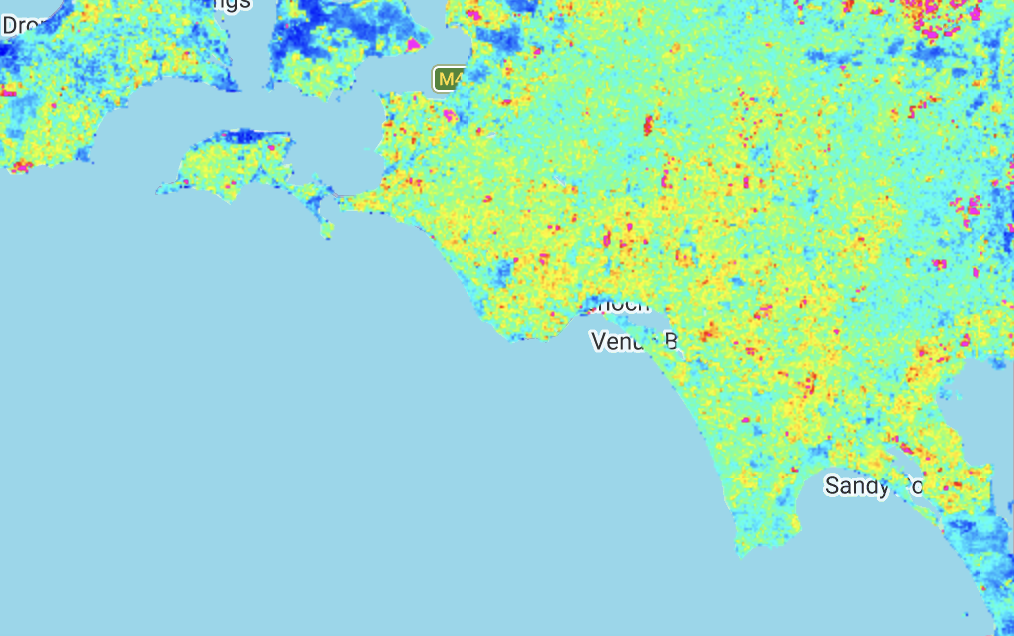
\includegraphics[width=0.8\textwidth]{fig1.png}
    \caption{Annual embedding-space change across the Bass Coast study area. Higher values indicate stronger environmental change between consecutive years.}
\end{figure}

\subsection{Hotspot Persistence Analysis}

To distinguish isolated disturbances from repeated environmental change, annual hotspot maps were aggregated through time to calculate hotspot persistence. Persistence represents the number of years that a pixel exceeded the selected hotspot threshold. Using the adopted threshold configuration, the analysis identified approximately 334.34 km$^2$ of long-term hotspot area between 2017 and 2024. When persistence criteria were applied, hotspot extent decreased substantially. Areas classified as hotspots in at least two years covered approximately 146.03 km$^2$, while areas classified as hotspots in at least three years covered approximately 57.20 km$^2$. These results suggest that although environmental change is relatively widespread, repeated or persistent change is concentrated within a much smaller subset of locations.

Figure~\ref{fig:persistence} illustrates the persistence-based hotspot mapping approach.

\begin{figure}[H]
    \centering
    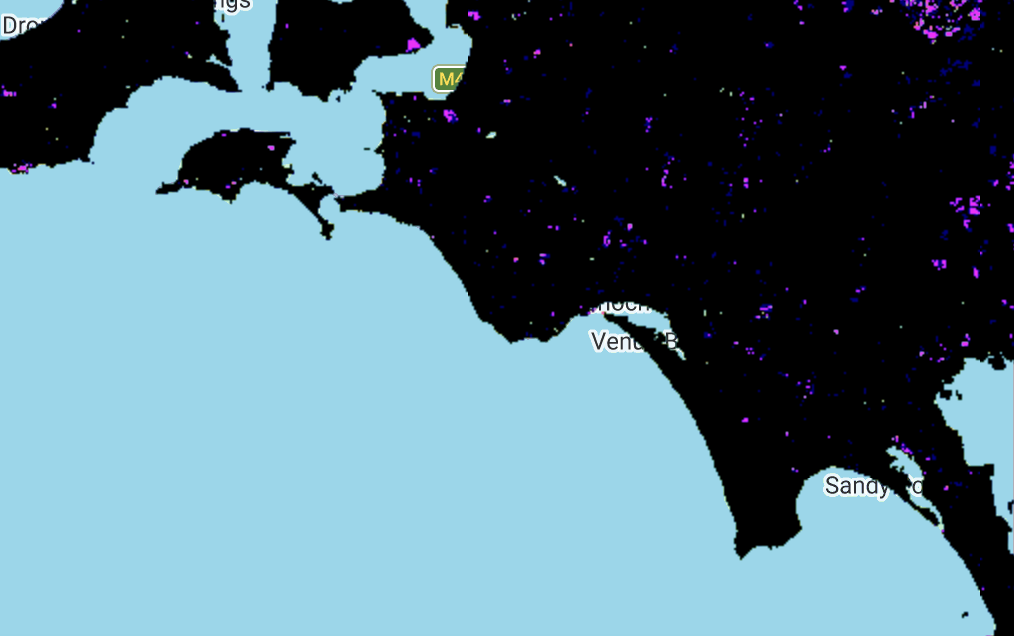
\includegraphics[width=0.8\textwidth]{fig2.png}
    \caption{Persistent hotspot locations derived from annual hotspot maps. Purple pixels indicate locations experiencing repeated environmental change across multiple years.}
    \label{fig:persistence}
\end{figure}

\subsection{Threshold Sensitivity Assessment}

A threshold sensitivity assessment was conducted to evaluate the influence of threshold selection on hotspot extent. In addition to the primary threshold configuration, alternative thresholds of 0.40 and 0.50 were tested. Lower thresholds resulted in a larger number of hotspot pixels being detected, while higher thresholds produced more conservative hotspot maps. At a threshold of 0.40, hotspot areas covered approximately 251.58 km$^2$ for persistence greater than or equal to two years and 108.36 km$^2$ for persistence greater than or equal to three years. Increasing the threshold to 0.50 reduced these areas to approximately 86.67 km$^2$ and 29.85 km$^2$, respectively. The consistency of this behavior demonstrated that hotspot extent responds predictably to threshold selection, providing confidence that the chosen thresholding strategy captures meaningful differences in environmental change intensity.

\begin{figure}[H]
    \centering
    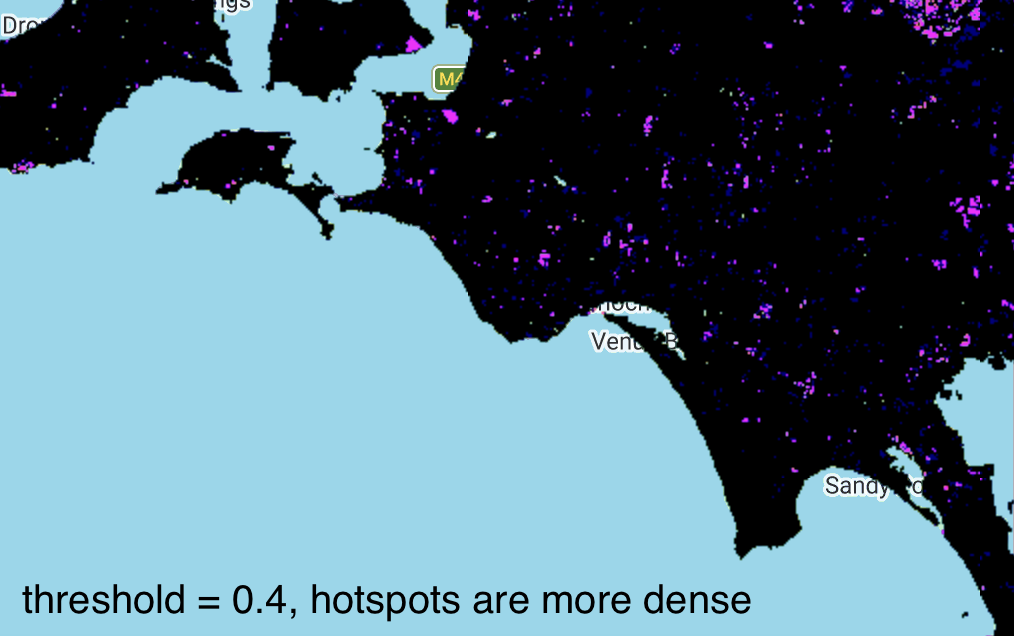
\includegraphics[width=0.48\textwidth]{fig3.png}
    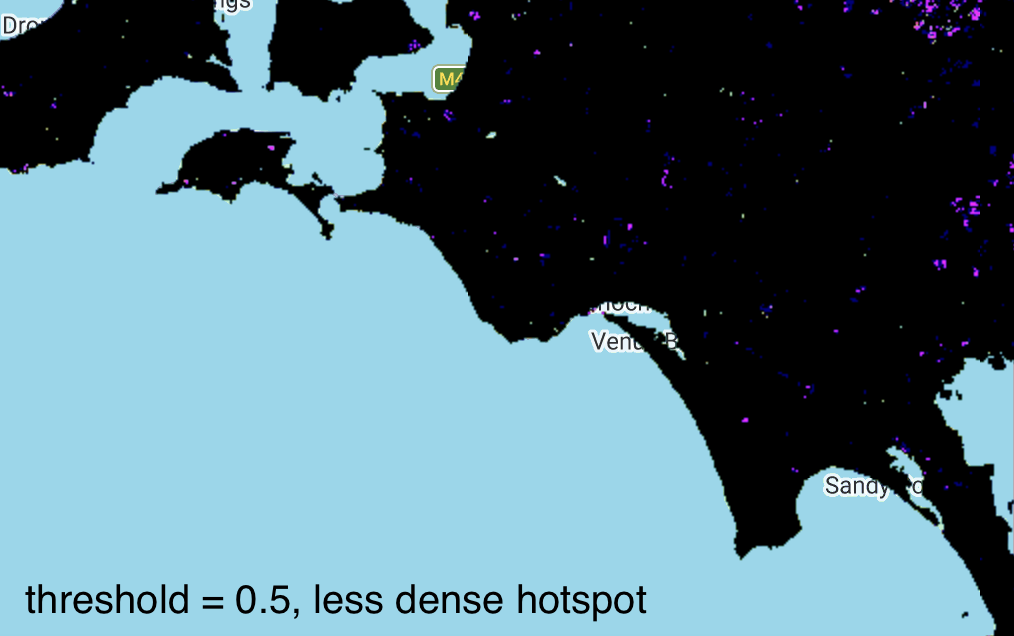
\includegraphics[width=0.48\textwidth]{fig4.png}
    \caption{Comparison of hotspot extent under alternative threshold configurations. Lower thresholds identify larger hotspot areas, while higher thresholds isolate only the strongest changes.}
\end{figure}

\section{Expansion of the Temporal Characterization Framework}

Following the initial hotspot mapping workflow, the temporal characterization framework was expanded to capture a broader range of landscape behaviours. While hotspot persistence provided a useful measure of repeated environmental change, it could not distinguish between locations undergoing gradual transitions, intermittent disturbances or isolated events. To address this limitation, annual time-series analysis and endpoint analysis were combined within the same workflow. Annual analysis was used to track how change evolved between consecutive years, while endpoint analysis compared the 2017 and 2024 embeddings directly to quantify total landscape transformation across the study period. Combining these two perspectives allowed both persistent change and one-off large transitions to be captured within the same framework.

Additional temporal metrics were derived from the annual change trajectory of each pixel. For each fixed pixel location, the annual embedding-distance sequence was defined as:

\[
D=
\left\{
d_{2017\rightarrow2018},
d_{2018\rightarrow2019},
d_{2019\rightarrow2020},
d_{2020\rightarrow2021},
d_{2021\rightarrow2022},
d_{2022\rightarrow2023},
d_{2023\rightarrow2024}
\right\}
\]

where each $(d_{y\rightarrow y+1})$ represents the Euclidean distance between the 64-dimensional embedding vector for year (y) and year (y+1) at the same pixel location. For example, a pixel with annual distances as:

\[[D = \{0.12, 0.50, 0.30, 0.60, 0.10, 0.55, 0.20\}\]

would be interpreted as having several years of stronger change mixed with years of lower change. The following metrics were then calculated from this annual distance sequence:

\begin{itemize}[leftmargin=*]

    \item \textbf{Persistence count.} Persistence count measures how many annual intervals exceeded the selected annual hotspot threshold (T). It was calculated as:

    \[P = \sum_{i=1}^{7} I(d_i > T)\]

    where $(I(\cdot))$ is an indicator function that returns 1 when the condition is true and 0 otherwise. In the current workflow, the annual threshold was set to (T = 0.45). Using the example above:

    \[D = \{0.12, 0.50, 0.30, 0.60, 0.10, 0.55, 0.20\}\]

    the values exceeding 0.45 are (0.50), (0.60), and (0.55), so the persistence count is:

    \[P = 3\]

    This means the pixel experienced strong annual change in three separate year intervals.

    \item \textbf{Cumulative change.} Cumulative change measures the total amount of annual change accumulated across the full period. It was calculated as:

    \[C = \sum_{i=1}^{7} d_i\]

    This metric is useful for identifying locations that may not exceed the hotspot threshold every year, but still accumulate substantial change over time.

    \item \textbf{Mean annual change.} Mean annual change summarizes the average annual embedding-space change for each pixel:

    \[\bar{d} = \frac{1}{7}\sum_{i=1}^{7} d_i\]

    This provides a simple measure of the typical annual change intensity at a location.

    \item \textbf{Maximum annual change.} Maximum annual change identifies the strongest single-year change event experienced by a pixel:

    \[d_{\max} = \max(D)\]

    This metric is useful for detecting sudden or high-magnitude transitions that may occur within a single year interval.

    \item \textbf{Variance of annual change.} Variance measures how much the annual change values fluctuate through time:

    \[\sigma^2 =
    \frac{1}{n-1}
    \sum_{i=1}^{n}
    (d_i-\bar{d})^2\]

    where (n=7) in the current annual sequence. High variance indicates that annual change is unstable or intermittent, with some years changing much more strongly than others. Low variance suggests a more consistent temporal pattern.

    \item \textbf{Slope of annual change.} Slope measures whether annual change intensity generally increases or decreases through time. To calculate this, each annual distance value was paired with a time index:

    \[x = \{1,2,3,4,5,6,7\}\]

    corresponding to the seven annual intervals from $(2017\rightarrow2018)$ through $(2023\rightarrow2024)$. A simple linear regression was then fitted for each pixel:

    \[d_i = \alpha + \beta x_i + \epsilon_i\]

    where $(d_i)$ is the annual embedding distance at time step (i), $(\alpha)$ is the intercept, $(\beta)$ is the slope, and $(\epsilon_i)$ is the residual error. The fitted slope $(\beta)$ was used as the slope metric:

    \[
    \beta =
    \frac{
    \sum_{i=1}^{n}
    (x_i-\bar{x})(d_i-\bar{d})
    }{
    \sum_{i=1}^{n}
    (x_i-\bar{x})^2
    }
    \]

    A positive slope indicates that annual change intensity is generally increasing over time, while a negative slope indicates that annual change intensity is generally decreasing. A slope close to zero suggests no strong directional trend in annual change intensity.

    \item \textbf{First hotspot year.} First hotspot year identifies the first annual interval in which a pixel exceeded the hotspot threshold. It was calculated as the first year (y+1) for which:

    \[d_{y \rightarrow y+1} > T\]

    For example, if the first threshold exceedance occurred in the $(2018\rightarrow2019)$ interval, the first hotspot year was recorded as 2019. Pixels that never exceeded the threshold were excluded from this metric.

    \item \textbf{Maximum change year.} Maximum change year identifies the year associated with the strongest annual change event. It was calculated from the annual interval with the largest embedding distance:

    \[
    y_{\max}
    =
    \arg\max_{y}
    \left(
    d_{y \rightarrow y+1}
    \right)
    \]

    In the implementation, this was recorded as the end year of the interval. For example, if the largest distance occurred between 2019 and 2020, the maximum change year was recorded as 2020.

\end{itemize}

Together, these metrics transformed the workflow from a hotspot detection framework into a temporal behavior characterization framework. Rather than simply identifying where change occurred, each pixel could now be described not only by the magnitude of change, but also by how that change evolved through time. This enabled the analysis to distinguish between different temporal patterns of environmental change, including persistent change, sudden disturbances, intermittent or variable behavior, increasing-change trends, decreasing-change trends and stable locations.

\begin{figure}[H]
    \centering
    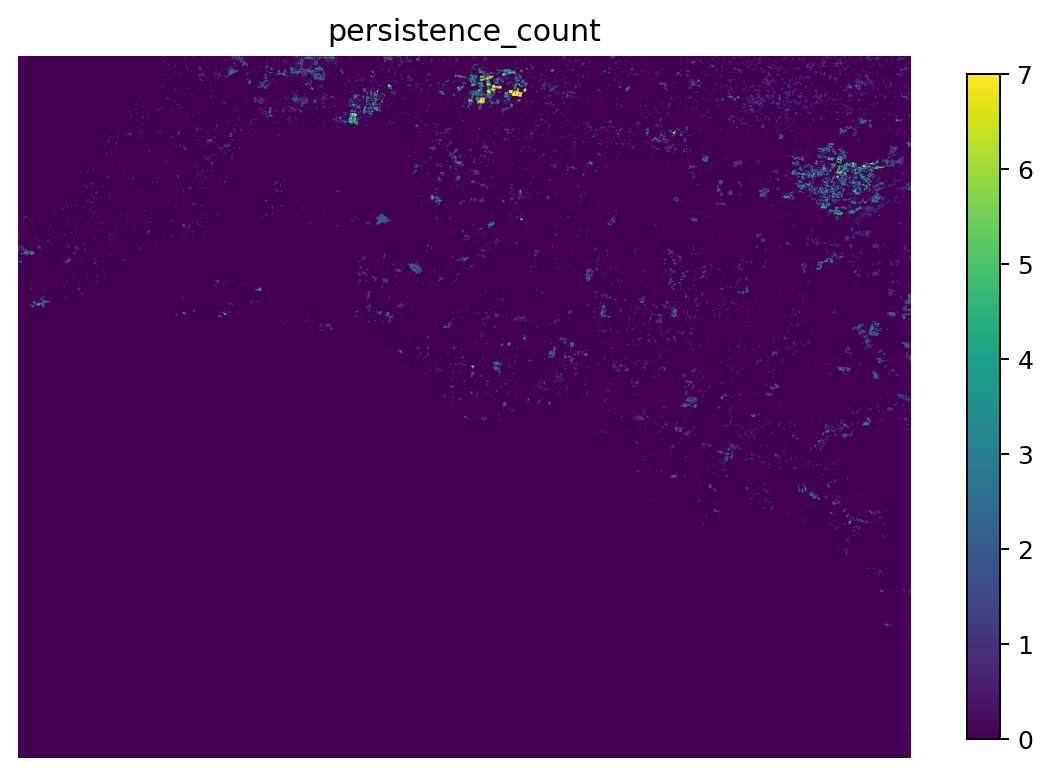
\includegraphics[width=0.75\textwidth]{fig5.png}
    \caption{Persistence count derived from annual hotspot maps. Higher values indicate locations that repeatedly exceeded the hotspot threshold through time.}
\end{figure}

\begin{figure}[H]
    \centering
    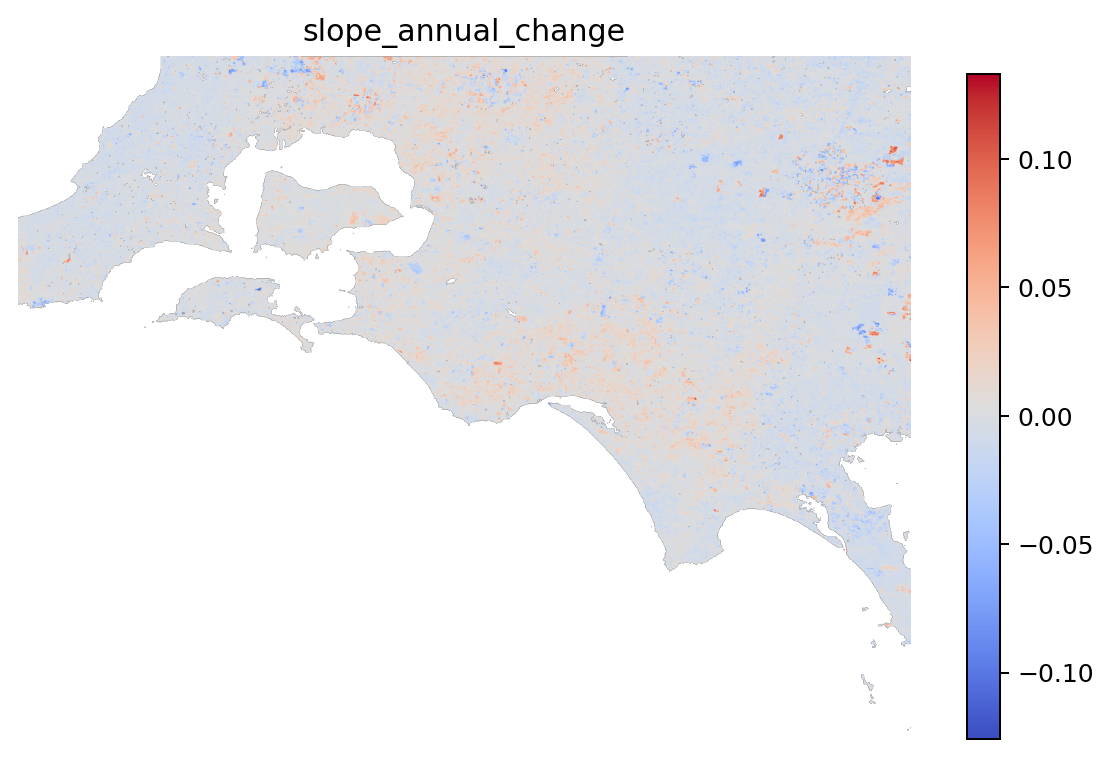
\includegraphics[width=0.75\textwidth]{fig6.png}
    \caption{Slope of annual change trajectories. Positive values indicate increasing change intensity through time, while negative values indicate decreasing change intensity.}
\end{figure}

\begin{figure}[H]
    \centering
    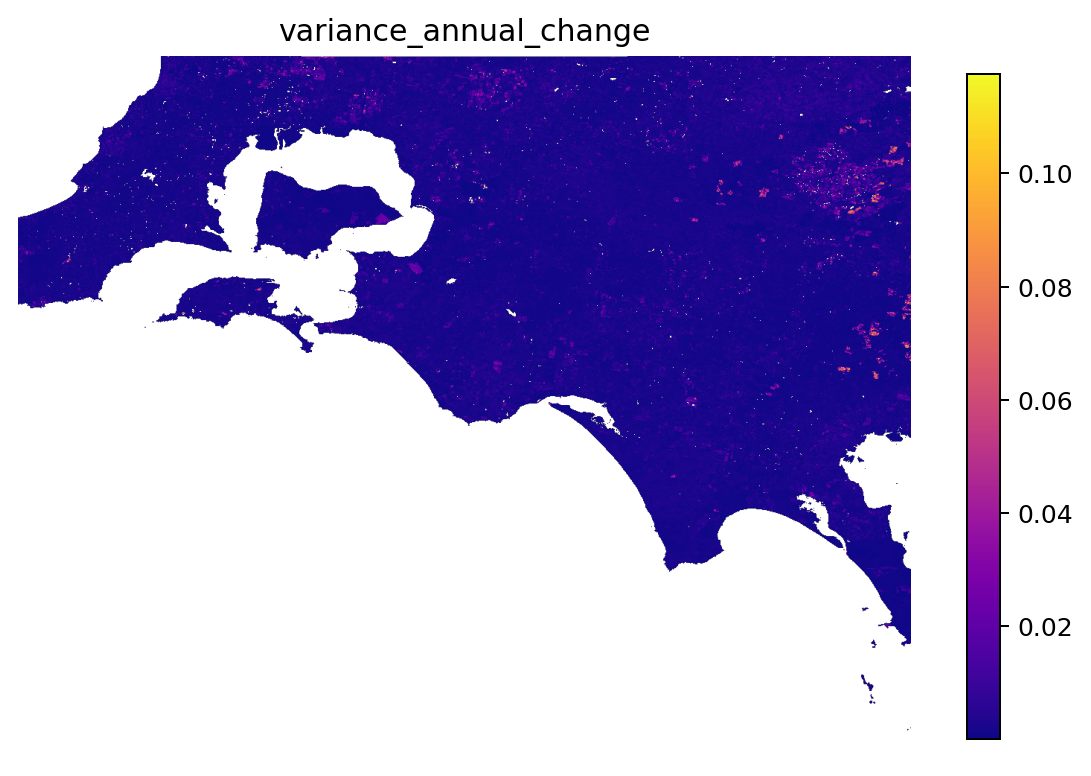
\includegraphics[width=0.75\textwidth]{fig7.png}
    \caption{Variance of annual change trajectories. Higher values indicate locations with more variable or unstable behavior through time.}
\end{figure}

\section{Transition to Python Workflow}

Following the development of the temporal characterization framework within Google Earth Engine, the next stage of the project focused on extracting the generated raster products and conducting more detailed local analysis in Python. The primary motivation for this transition was computational flexibility. While Google Earth Engine provided an efficient environment for generating annual change products and hotspot maps, it became increasingly restrictive for large-scale exploratory analysis, custom visualization and pixel-level investigation. The exported dataset consisted of multiple GeoTIFF layers describing different aspects of landscape behavior, including endpoint change, persistence count, cumulative change, variance, slope, first hotspot year and maximum change year. Initial attempts to load and analyze these datasets directly revealed practical limitations associated with raster size and memory consumption. Several of the exported products contained millions of pixels, making full in-memory processing inefficient and difficult to scale. To address this challenge, a window-based processing strategy was adopted. Rather than loading complete rasters into memory, the workflow processed data in smaller spatial blocks while preserving full coverage of the study area. This significantly reduced memory requirements and allowed large datasets to be analyzed efficiently on local hardware. The resulting Python workflow provided a more flexible environment for statistical analysis, visualization and future integration with external interpretation datasets.

\section{Raster Exploration and Validation}

The first phase of local analysis focused on validating the exported Earth Engine products before proceeding to more advanced interpretation. The objective was to ensure that all raster outputs were correctly generated, spatially aligned and suitable for downstream analysis. A series of quality-control checks were performed across all exported layers. These included verifying raster dimensions, coordinate systems, spatial alignment, no-data handling and annual product availability. Summary statistics and distribution plots were also generated to inspect the numerical behavior of each metric and identify any unexpected artefacts. The validation process confirmed that all exported rasters loaded correctly and remained spatially consistent across the study area. Annual outputs were available for all expected years and no significant alignment issues were identified. Distribution analysis further showed that the derived metrics behaved as expected, with most locations exhibiting relatively low to moderate change and a smaller subset of pixels occupying the upper tail of the distribution.

Figure~\ref{fig:endpoint_map} shows the endpoint change product generated from the comparison between 2017 and 2024. Most of the study area exhibited relatively modest levels of change, while stronger transformations appeared as localized clusters distributed across the landscape.

\begin{figure}[H]
    \centering
    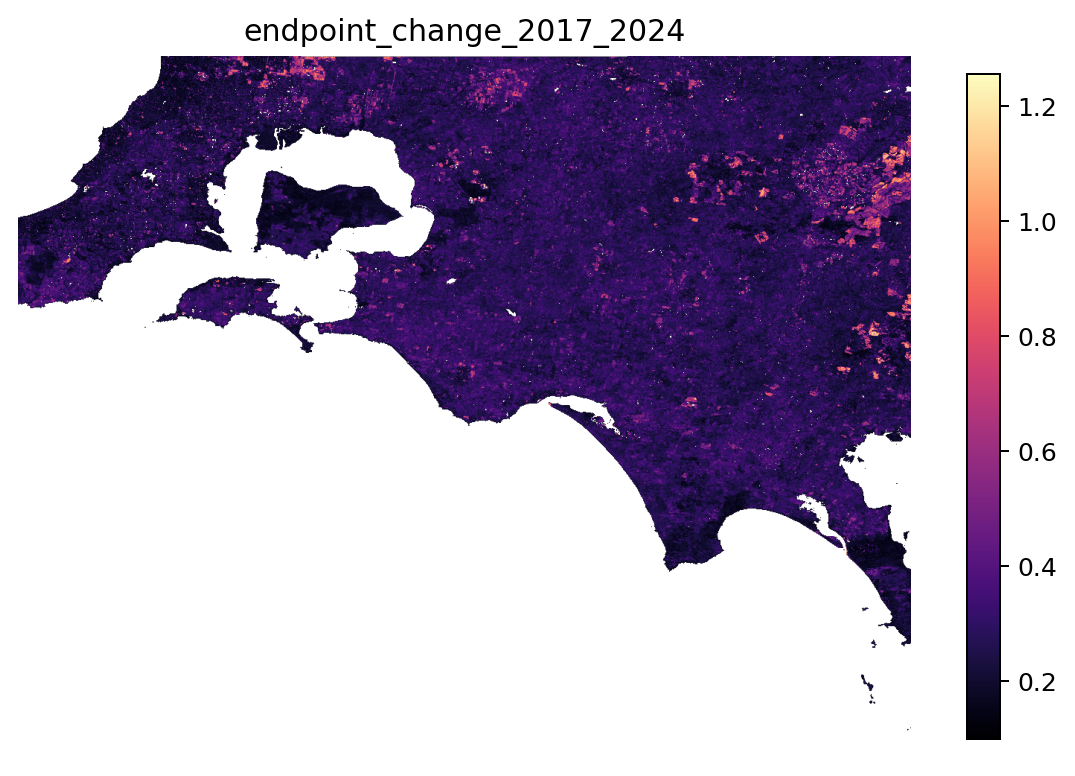
\includegraphics[width=0.70\textwidth]{fig8.png}
    \caption{Endpoint change between 2017 and 2024 derived from Satellite Embedding V1. Higher values indicate stronger overall landscape transformation across the study period.}
    \label{fig:endpoint_map}
\end{figure}

The distribution of endpoint change values is shown in Figure~\ref{fig:endpoint_hist}. The strongly right-skewed distribution supports the use of percentile-based thresholding, where only the most extreme change values are classified as hotspots.

\begin{figure}[H]
    \centering
    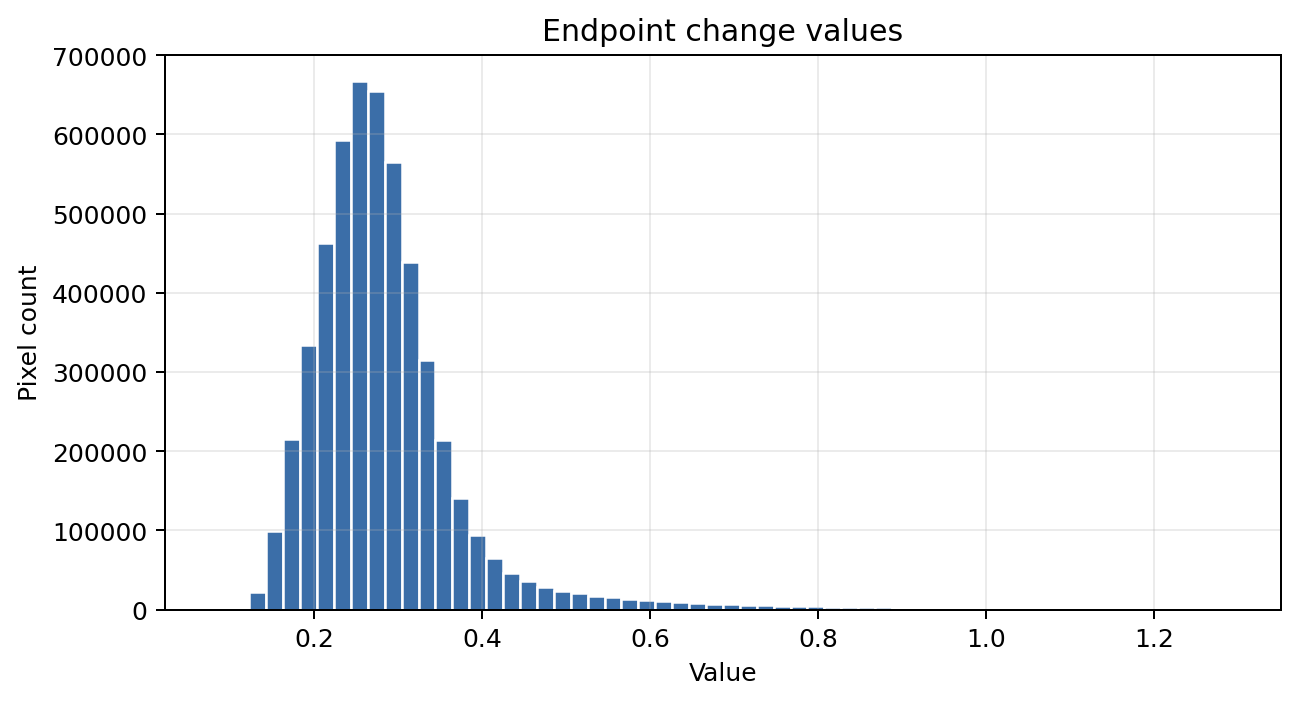
\includegraphics[width=0.75\textwidth]{fig9.png}
    \caption{Distribution of endpoint change values across the study area. Most pixels exhibit relatively low change, while a smaller subset forms a long upper tail representing stronger landscape transformation.}
    \label{fig:endpoint_hist}
\end{figure}

Overall, the raster validation stage established confidence in the integrity of the exported products and confirmed that the temporal metrics were suitable for further behavioral analysis.

\section{Behavioral Characterization and Hypothesis Testing}

This part of the analysis focused on evaluating whether the temporal metrics derived from the satellite embeddings could distinguish different types of landscape behavior. The working hypothesis was:

\begin{quote}
\emph{Different temporal landscape behaviors should produce distinguishable signatures within the embedding-derived metric space.}
\end{quote}

To test this hypothesis, the raster products generated during the previous stages were converted into a sampled pixel-level dataset. For each sampled location, a range of temporal metrics was extracted, including endpoint change, persistence count, cumulative change, mean annual change, maximum annual change, variance, slope, first hotspot year and maximum change year. These metrics were then used to define a set of rule-based behavioral categories designed to represent different temporal patterns of environmental change. Importantly, these categories were not intended to represent specific ecological processes or land-cover classes. Instead, they were designed as behavioral archetypes that could be used to test whether the proposed temporal metrics captured meaningful differences in how landscape change evolves through time.

Table~\ref{tab:behaviour_categories} summarises the behavioural categories used in the analysis.

\begin{table}[H]
\centering
\caption{Rule-based behavioural categories used for hypothesis testing.}
\label{tab:behaviour_categories}
\renewcommand{\arraystretch}{1.25}
\begin{tabularx}{\textwidth}{>{\raggedright\arraybackslash}p{3.5cm} X}
\toprule
\textbf{Category} & \textbf{Definition} \\
\midrule

Endpoint hotspot &
Pixels located within the long-term endpoint hotspot mask for 2017--2024. \\

Persistent ($\geq$2) &
Pixels with persistence count greater than or equal to two years. \\

Persistent ($\geq$3) &
Pixels with persistence count greater than or equal to three years. \\

High variance &
Pixels within the upper 5\% of variance values, representing highly variable or intermittent annual change behaviour. \\

Positive slope &
Pixels within the upper 5\% of slope values, representing locations where annual change intensity generally increased through time. \\

Negative slope &
Pixels within the lower 5\% of slope values, representing locations where annual change intensity generally decreased through time. \\

Sudden-change candidate &
Pixels with high endpoint change but low persistence, indicating a large cumulative change driven by one or a small number of annual events. \\

Temporary or recovery candidate &
Pixels with relatively low endpoint change but high variance, indicating fluctuating behaviour that may represent temporary disturbance, recovery or oscillating environmental conditions. \\

Stable control &
Pixels with low endpoint change, zero persistence, low variance and slope values close to zero. \\

\bottomrule
\end{tabularx}
\end{table}

Using these behavioural definitions, a balanced sample of pixels was extracted from each category and analysed using boxplots, scatter plots and summary statistics. The objective was to determine whether the categories occupied distinct regions of the metric space or whether they collapsed into a common distribution.

The results provided strong support for the proposed hypothesis. Behavioural categories consistently exhibited different statistical characteristics across multiple metrics. Stable-control pixels remained concentrated within low-change regions of the metric space, while persistent-change categories exhibited substantially higher persistence values and elevated endpoint change scores. Sudden-change candidates displayed relatively large endpoint changes despite low persistence counts, supporting the expectation that isolated disturbances produce a different temporal signature from long-term environmental change.

Figure~\ref{fig:endpoint_category} shows the distribution of endpoint change across the behavioural categories. Persistent-change and sudden-change categories generally occupied higher endpoint-change ranges than stable-control locations, while high-variance and slope-based categories occupied intermediate regions of the distribution. The separation between categories indicates that endpoint change captures meaningful differences in cumulative landscape transformation.

\begin{figure}[H]
    \centering
    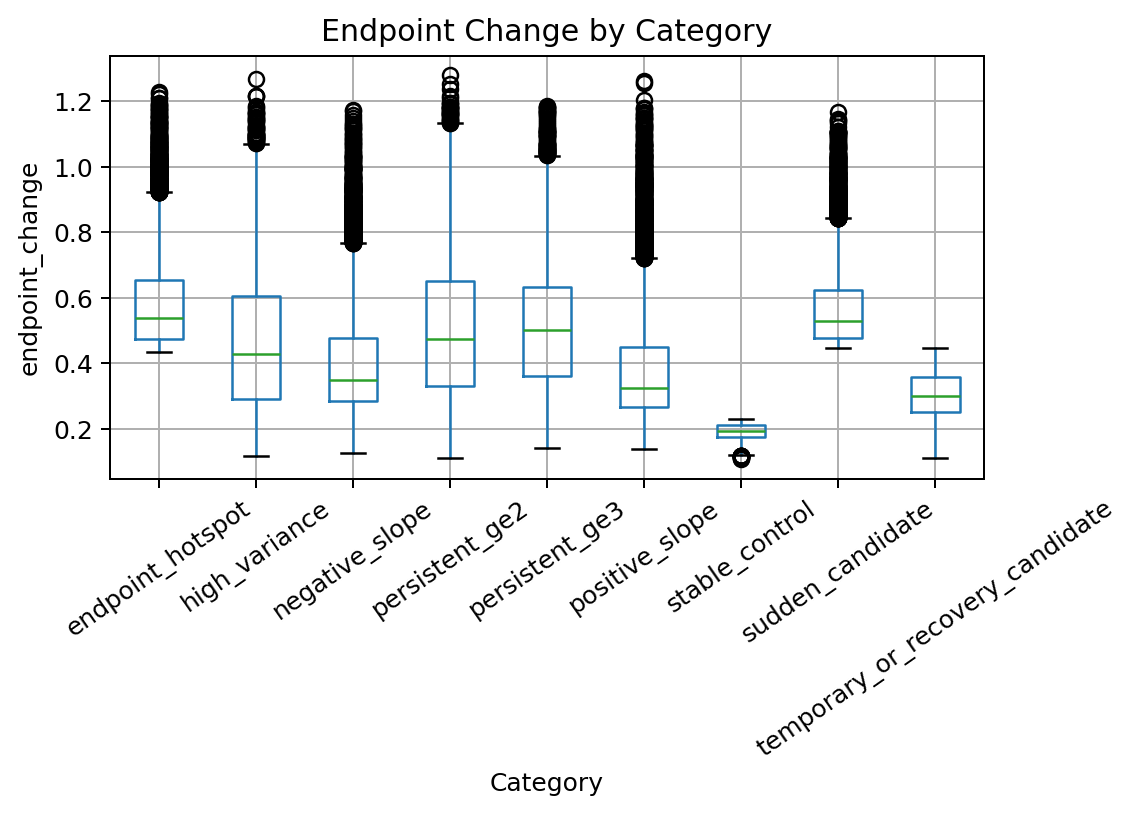
\includegraphics[width=0.75\textwidth]{fig10.png}
    \caption{Distribution of endpoint change across behavioural categories. Distinct distributions indicate that different landscape behaviours occupy different regions of the embedding-derived metric space.}
    \label{fig:endpoint_category}
\end{figure}

Figure~\ref{fig:persistence_category} presents the corresponding persistence distributions. As expected, persistent-change categories exhibit substantially higher persistence values than stable-control and sudden-change categories. The clear separation observed across persistence counts provides additional evidence that repeated environmental change can be distinguished from isolated events using the proposed temporal metrics.

\begin{figure}[H]
    \centering
    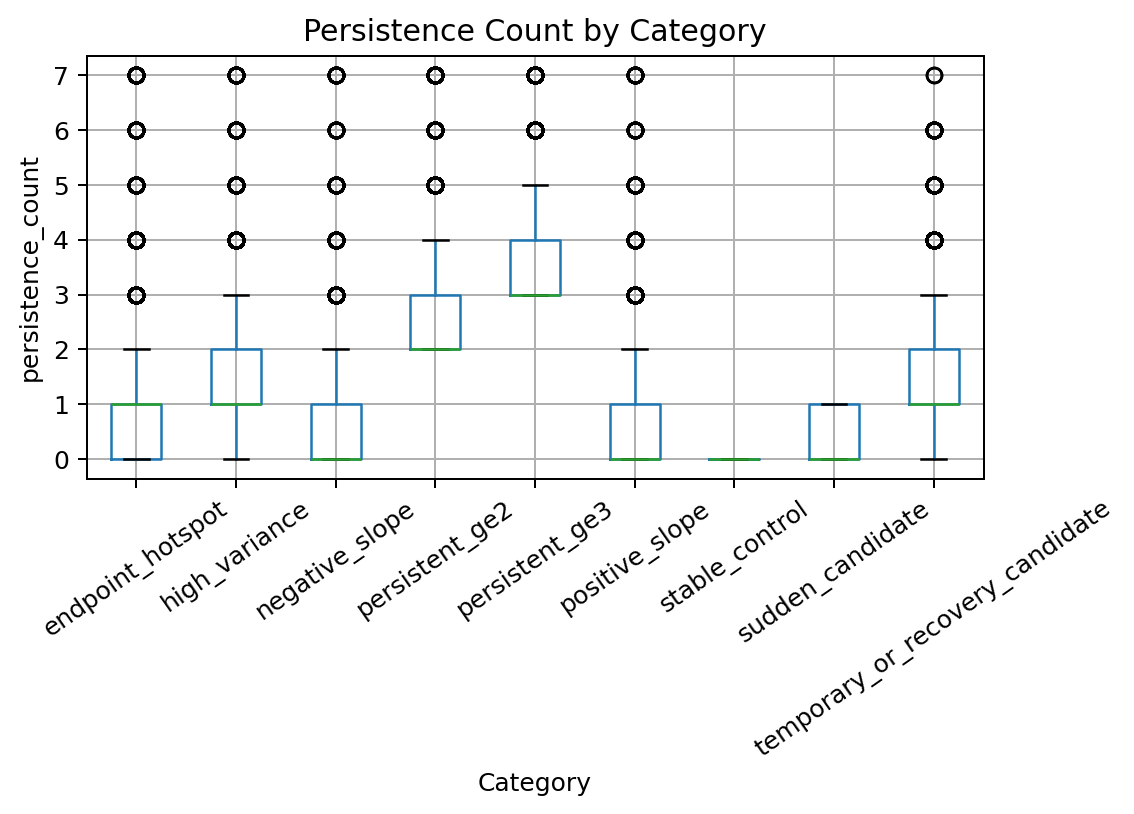
\includegraphics[width=0.75\textwidth]{fig11.png}
    \caption{Persistence count across behavioural categories. Persistent-change groups exhibit higher persistence values than stable or transient categories, supporting the behavioural interpretation framework.}
    \label{fig:persistence_category}
\end{figure}

Overall, the behavioural categories occupied distinct regions of the metric space rather than collapsing into a single distribution. This demonstrates that the embedding-derived temporal metrics contain meaningful information about how environmental change evolves through time. The results support the working hypothesis and establish a foundation for the next stage of the project, where these behavioural signatures will be linked with external datasets to investigate their ecological interpretation and real-world significance.

\section{Integration of DEA Land Cover for External Context}

The embedding-derived metrics developed in the previous sections provide a detailed description of where change occurred and how the strength of that change evolved through time. However, the embedding metrics do not directly assign semantic land-cover labels to each location. A high endpoint-change value or a persistent hotspot indicates that the encoded land-surface characteristics changed, but it does not by itself identify whether the location changed from natural vegetation to cultivated vegetation, from vegetation to artificial surface, or between other broad land-cover states. For this reason, an external contextual dataset was required to support interpretation of the behavioural categories.

Digital Earth Australia (DEA) Land Cover was selected as the first external interpretation layer because it provides annual land-cover information across Australia over the same period as the embedding analysis. In this project, DEA Land Cover was used as an independent source of broad land-cover history for the Bass Coast study area. The purpose was not to replace the embedding-based change detection framework, but to provide additional context for interpreting the types of land-cover transitions that occur within embedding-derived hotspots and behavioural categories.

DEA Land Cover provides multiple levels of thematic detail. In this analysis, Level 3 and Level 4 classes were used. Level 3 represents broad land-cover groups, such as natural terrestrial vegetation, cultivated terrestrial vegetation, artificial surface, natural bare surface and water. Level 4 provides a more detailed subdivision of these broader classes, including distinctions such as woody and herbaceous vegetation structure. Level 3 was used as the main interpretation level because it is more stable and easier to summarize across the full study area, while Level 4 was retained as a more detailed supporting layer. This distinction is important because the objective of the current stage was to evaluate broad land-cover histories rather than assign highly specific ecological causes to individual pixels.

Figure~\ref{fig:dea_level3_2017_2024} shows DEA Level 3 land-cover classes for the Bass Coast study area at the beginning and end of the analysis period. The figure illustrates the type of external contextual information provided by DEA Land Cover. While the embedding workflow measures change in high-dimensional feature space, DEA Land Cover provides broad categorical labels that can be compared through time and linked back to the embedding-derived behavioural categories.

\begin{figure}[H]
    \centering
    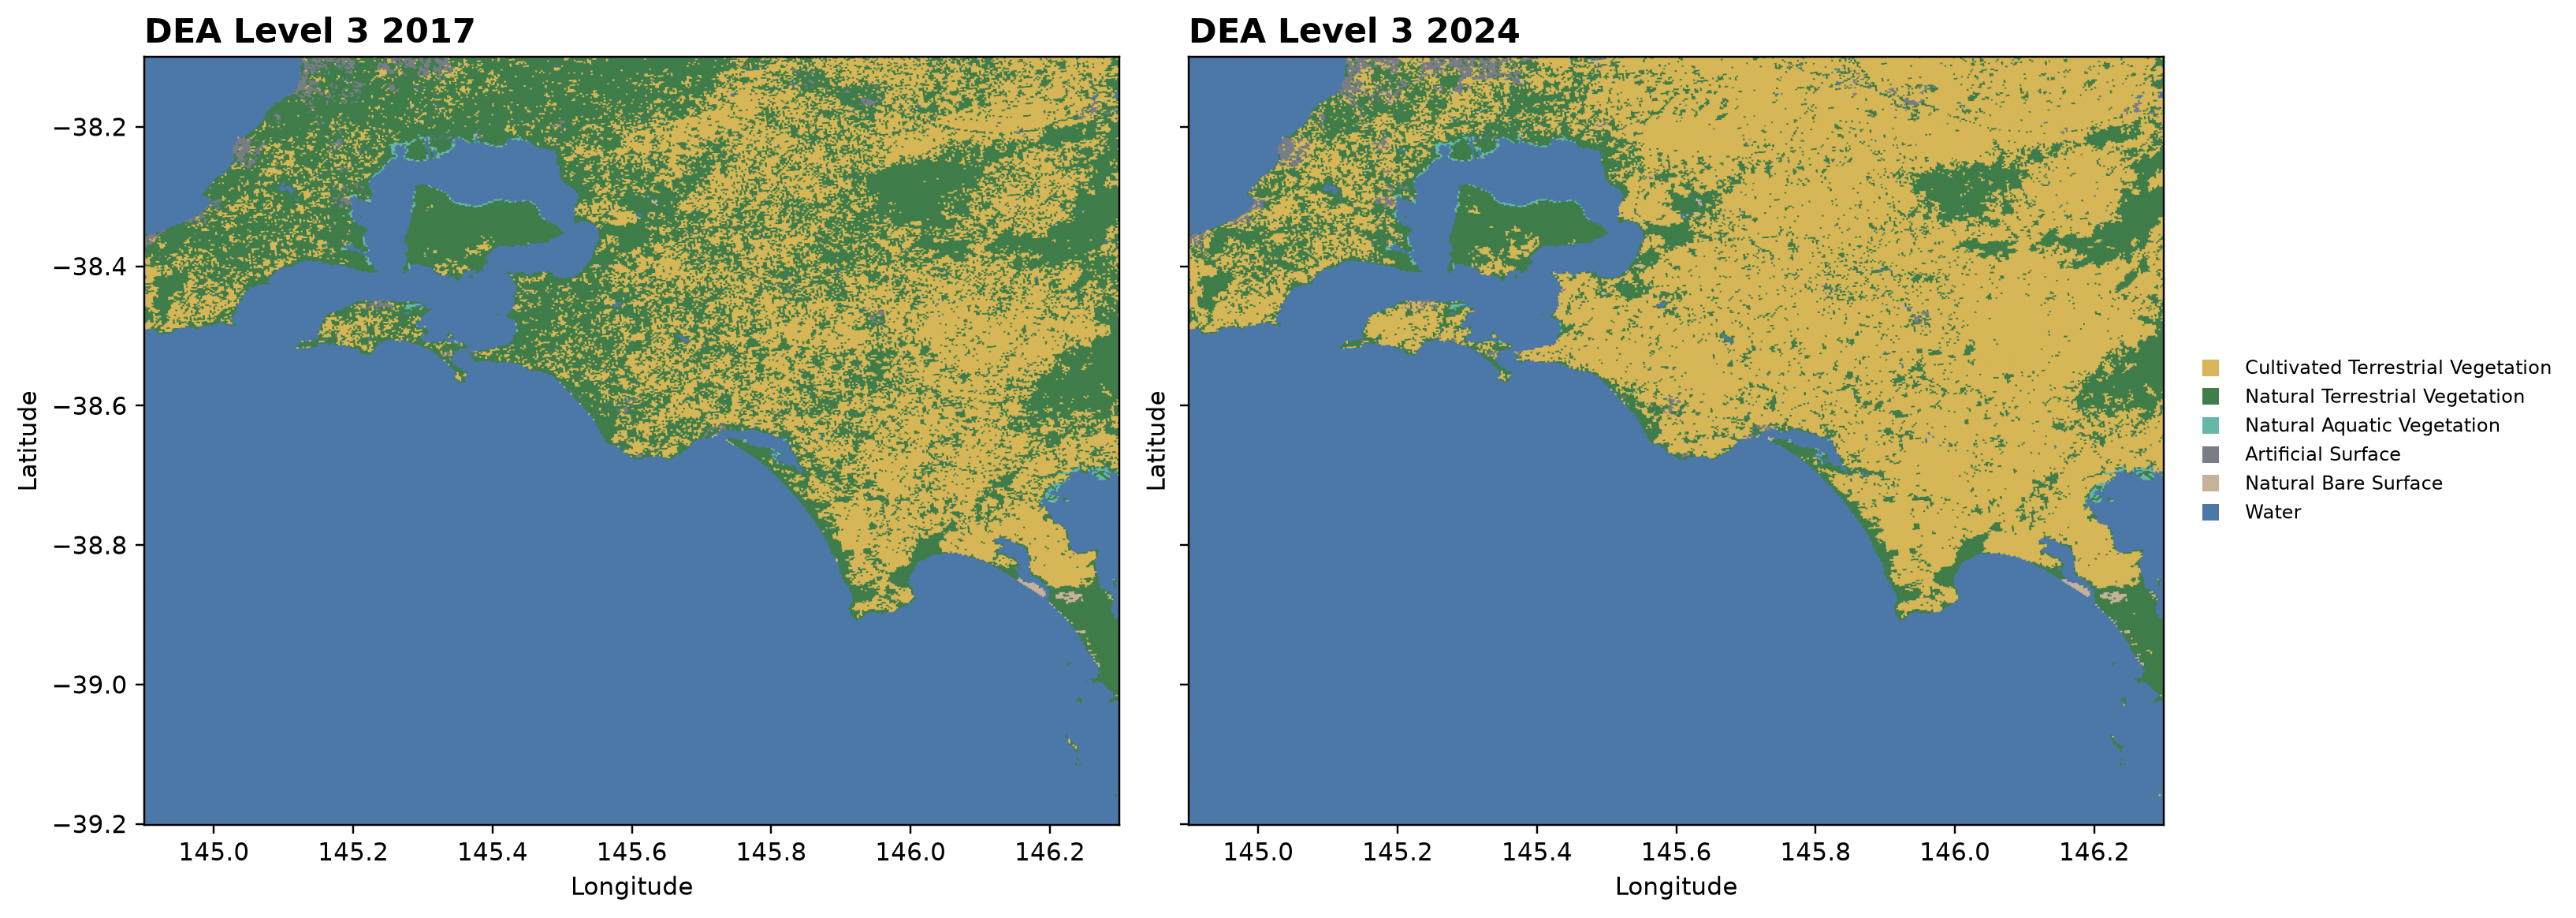
\includegraphics[width=0.95\textwidth]{fig12.png}
    \caption{DEA Land Cover Level 3 classes for the Bass Coast study area in 2017 and 2024. These broad land-cover classes provide external context for interpreting embedding-derived change signals.}
    \label{fig:dea_level3_2017_2024}
\end{figure}

\section{Sample-Based DEA Land Cover Enrichment}

After establishing that the embedding-derived behavioural categories occupied distinct regions of the metric space, the next step was to test whether these categories were also associated with independent land-cover histories. This was first conducted using a sampled pixel-level dataset rather than the full raster stack. The full Bass Coast raster contains a very large number of valid pixels, making it inefficient and unnecessary to flatten every pixel into a table for exploratory interpretation. Instead, a stratified sample was created from the behavioural categories defined earlier in the report. The final sampled dataset contained 89,707 points across the behavioural categories, allowing each category to be represented by a manageable number of points while preserving the ability to compare categories in a consistent way.

For each sampled location, the pixel coordinate was linked with annual DEA Land Cover labels from 2017 to 2024. This produced a land-cover sequence for each point. For example, a point could remain classified as natural terrestrial vegetation across all years, change from natural terrestrial vegetation to cultivated terrestrial vegetation, or move through a more variable sequence before returning to its original class. These DEA sequences were then summarized in several ways. First, the 2017 and 2024 DEA labels were compared to identify endpoint transitions. Second, the full annual sequence was examined to determine whether each point remained stable, changed once, changed temporarily and returned to its starting class, or moved into another broad land-cover group. Third, the first year of DEA-observed change was compared with embedding-derived timing metrics such as maximum change year and first hotspot year.

The sample-based analysis provided an important bridge between embedding-space behaviour and external land-cover context. The results showed that embedding-derived change categories had substantially higher rates of DEA-observed land-cover change than stable-control locations. For example, categories such as positive slope, persistent change and endpoint hotspot exhibited much higher Level 3 change shares than the stable-control category. This does not mean that DEA Land Cover provides an accuracy score for the embedding model. Instead, it indicates that the embedding-derived behavioural categories are enriched for independent land-cover change signals relative to stable locations.

\begin{table}[H]
\centering
\caption{Sample-based DEA Land Cover enrichment results for selected behavioural categories. The Level 3 changed share represents the proportion of sampled points in each category that experienced at least one DEA Level 3 class change between 2017 and 2024.}
\label{tab:dea_sample_enrichment}
\renewcommand{\arraystretch}{1.2}
\begin{tabularx}{0.85\textwidth}{>{\raggedright\arraybackslash}X r}
\toprule
\textbf{Behavioural category} & \textbf{DEA Level 3 changed share} \\
\midrule
Positive slope & 75.5\% \\
Persistent ($\geq$3) & 74.4\% \\
Persistent ($\geq$2) & 71.8\% \\
Temporary or recovery candidate & 68.4\% \\
High variance & 68.2\% \\
Negative slope & 65.8\% \\
Endpoint hotspot & 64.8\% \\
Sudden-change candidate & 61.6\% \\
Stable control & 29.9\% \\
\bottomrule
\end{tabularx}
\end{table}

The contrast between the change-oriented categories and the stable-control category supports the interpretation that the embedding-derived temporal metrics are capturing meaningful landscape dynamics. At the same time, the results must be interpreted carefully. DEA Land Cover provides broad annual land-cover classes, and therefore it can describe general transitions such as natural vegetation to cultivated vegetation or vegetation to artificial surface. It does not, on its own, prove the specific cause of a change event. The sample-based enrichment analysis therefore served as a validation and interpretation step: it demonstrated that the behavioural categories derived from Satellite Embedding V1 are associated with independent land-cover histories, while preserving a clear distinction between change detection, land-cover labelling and causal interpretation.

\section{Wall-to-Wall DEA Land Cover Summary}

The sample-based DEA analysis provided an efficient way to test whether the behavioural categories were associated with independent land-cover histories. However, the sampled analysis did not provide a complete spatial summary of all pixels in each category. To address this, the workflow was extended to a wall-to-wall summary across the Bass Coast raster stack. The objective of this stage was to summarize DEA Land Cover histories for all pixels matching each embedding-derived behavioural category, while avoiding the creation of an extremely large pixel-level table.

The wall-to-wall analysis used a raster-window processing strategy. Rather than converting the full raster into a row for every pixel, the rasters were processed in spatial blocks. For each block, the relevant embedding-derived metrics were read, the behavioural category masks were reconstructed, and the corresponding annual DEA Land Cover labels were summarized. This allowed the analysis to cover the full study area while producing compact summary tables rather than a very large pixel-level export. The approach is consistent with the memory-safe processing strategy used earlier in the Python workflow.

Because the embedding products and DEA Land Cover are not provided at the same spatial resolution, the DEA labels were aligned to the embedding raster grid using nearest-neighbour resampling for summary purposes. This allowed the embedding-derived category masks to remain fixed while assigning each embedding-grid pixel a corresponding DEA land-cover label. The resulting summaries should therefore be interpreted as broad land-cover context associated with the embedding grid, rather than as a claim that DEA provides independent 10 m land-cover classification.

The wall-to-wall results were consistent with the sample-based analysis. Figure~\ref{fig:dea_change_share_wall_to_wall} shows the proportion of pixels in each behavioural category that experienced at least one DEA class change between 2017 and 2024. Change-oriented categories had substantially higher DEA Level 3 changed shares than the stable-control category. For example, positive-slope pixels had a Level 3 changed share of approximately 75.3\%, persistent pixels with persistence greater than or equal to three years had a changed share of approximately 74.0\%, and endpoint hotspots had a changed share of approximately 64.7\%. In comparison, stable-control pixels had a Level 3 changed share of approximately 30.0\%.

\begin{figure}[H]
    \centering
    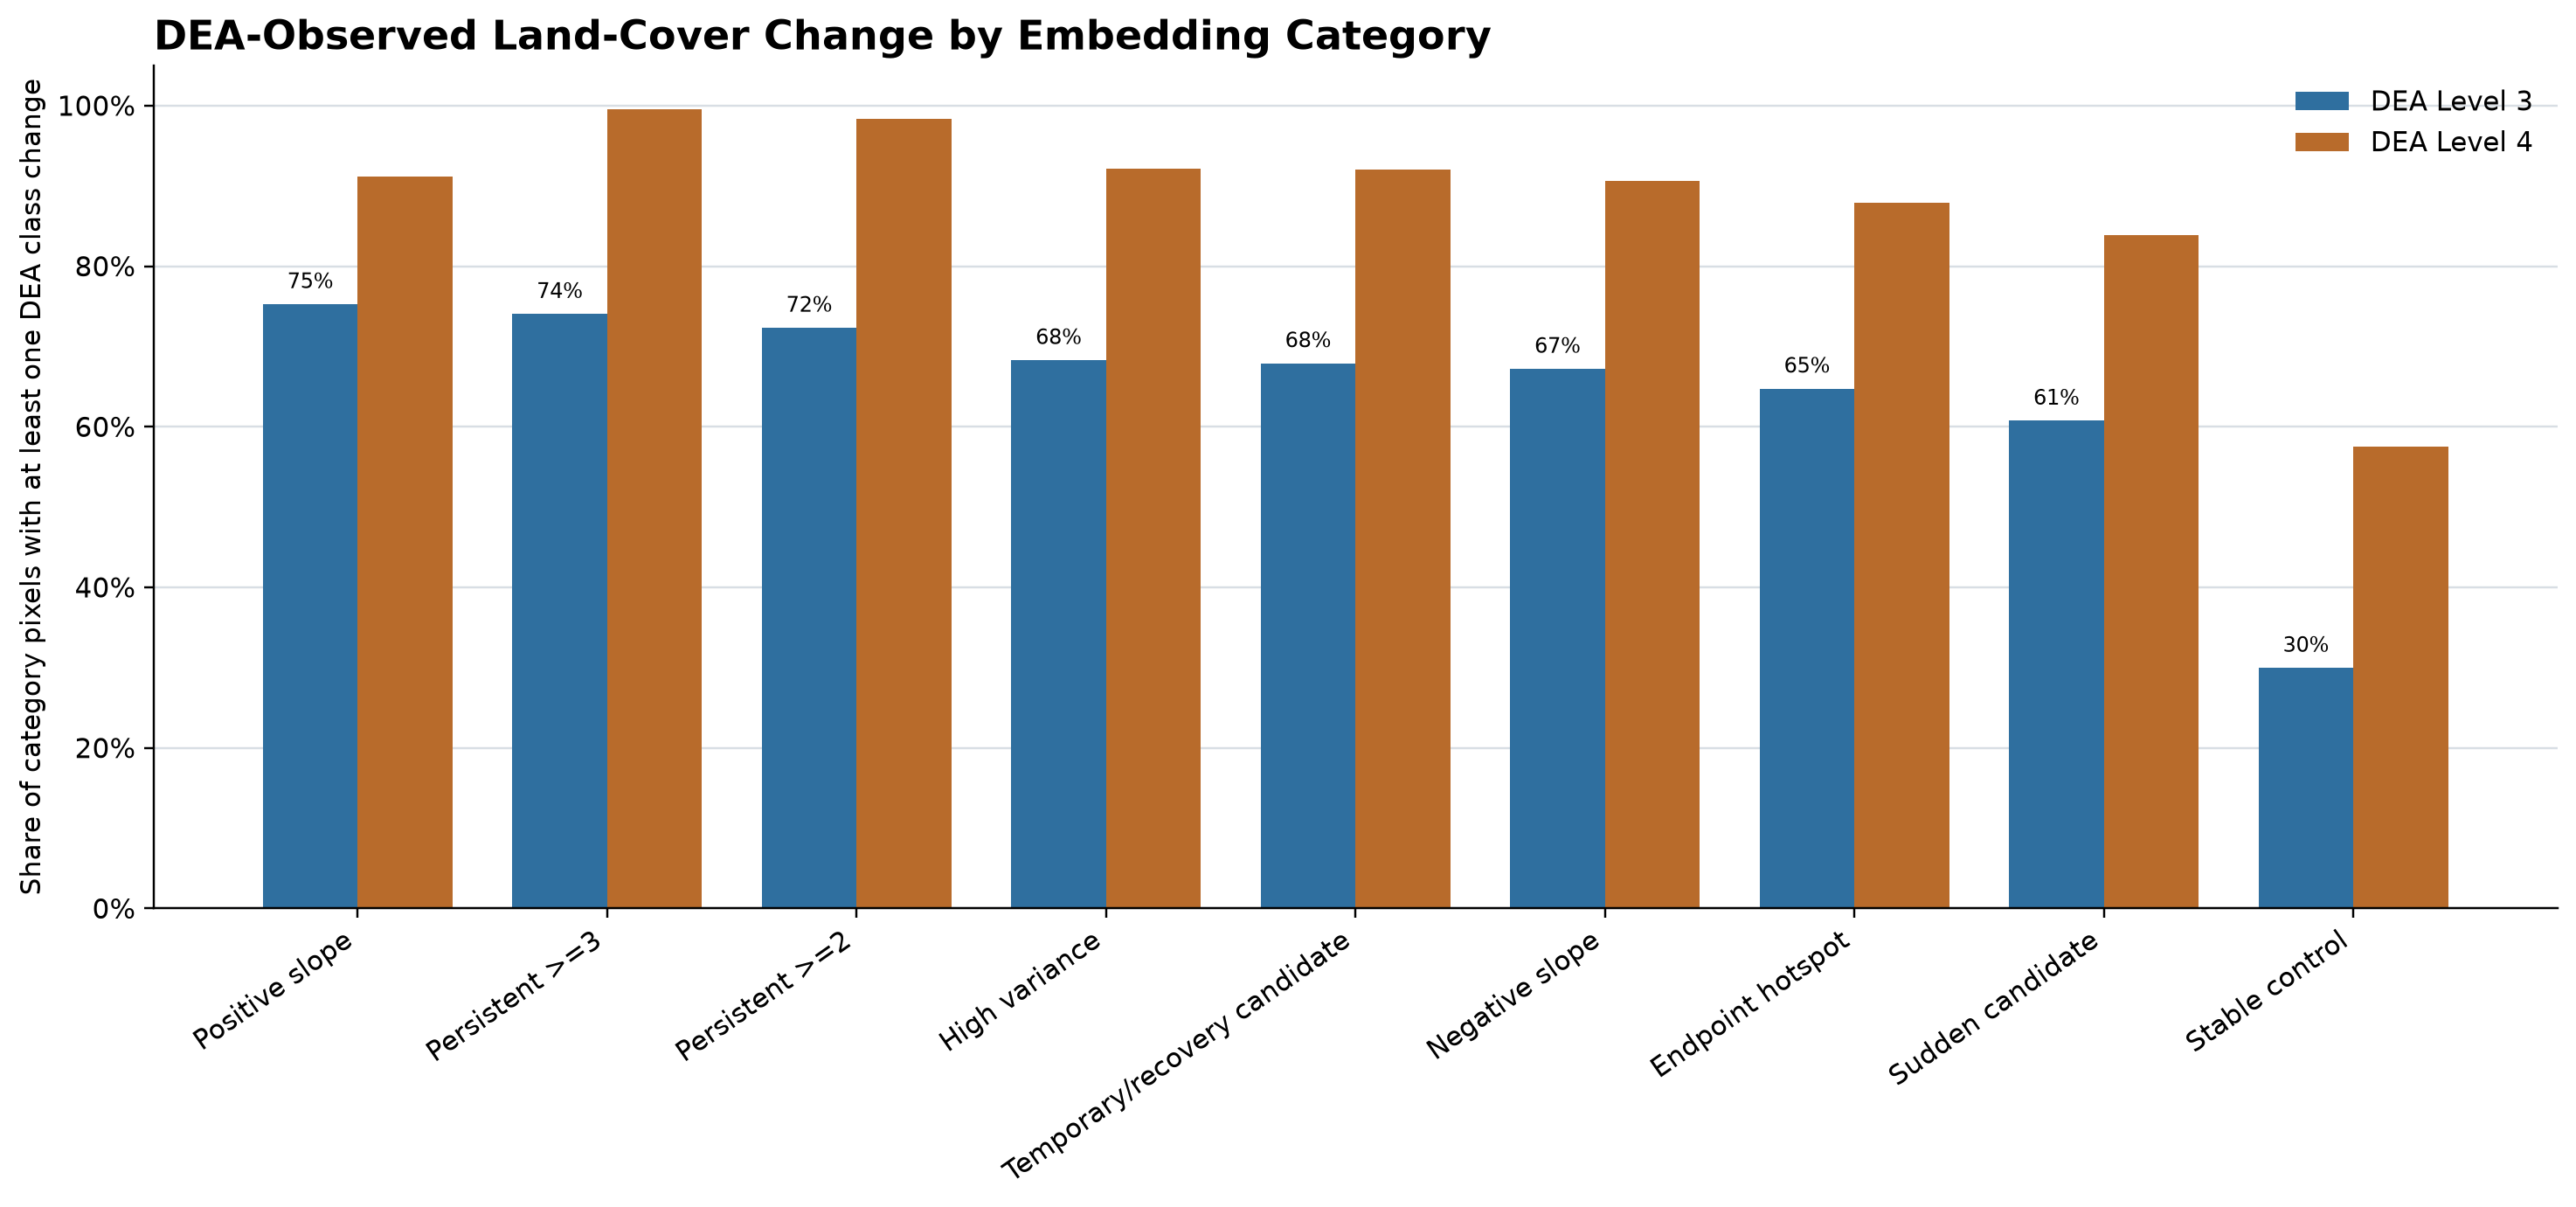
\includegraphics[width=0.95\textwidth]{fig13.png}
    \caption{Wall-to-wall DEA-observed land-cover change share by embedding-derived behavioural category. Change-oriented categories show substantially higher DEA Level 3 and Level 4 changed shares than the stable-control category.}
    \label{fig:dea_change_share_wall_to_wall}
\end{figure}

Table~\ref{tab:dea_wall_to_wall_summary} summarizes the wall-to-wall DEA Level 3 changed share for each behavioural category. These values should be interpreted as enrichment signals rather than accuracy scores. They describe how frequently pixels in each embedding-derived category were associated with at least one broad DEA Level 3 class change during the study period.

\begin{table}[H]
\centering
\caption{Wall-to-wall DEA Level 3 changed share by embedding-derived behavioural category across the Bass Coast study area.}
\label{tab:dea_wall_to_wall_summary}
\renewcommand{\arraystretch}{1.2}
\begin{tabularx}{0.9\textwidth}{>{\raggedright\arraybackslash}X r r}
\toprule
\textbf{Behavioural category} & \textbf{Pixel count} & \textbf{DEA Level 3 changed share} \\
\midrule
Positive slope & 4,153,371 & 75.3\% \\
Persistent ($\geq$3) & 781,578 & 74.0\% \\
Persistent ($\geq$2) & 1,992,917 & 72.3\% \\
High variance & 4,149,329 & 68.3\% \\
Temporary or recovery candidate & 2,150,815 & 67.9\% \\
Negative slope & 4,156,136 & 67.2\% \\
Endpoint hotspot & 4,550,716 & 64.7\% \\
Sudden-change candidate & 3,064,197 & 60.8\% \\
Stable control & 3,484,658 & 30.0\% \\
\bottomrule
\end{tabularx}
\end{table}

The behavioural categories are not mutually exclusive. A pixel can satisfy more than one rule, such as being both an endpoint hotspot and a high-variance pixel. For this reason, the pixel counts in Table~\ref{tab:dea_wall_to_wall_summary} should be interpreted category by category and should not be summed as a total area estimate across Bass Coast.

The close agreement between the sampled analysis and the wall-to-wall summary provided additional confidence in the stability of the results. Figure~\ref{fig:sample_wall_to_wall_comparison} compares the Phase 3 sampled estimates with the Phase 5 wall-to-wall estimates. The similarity between the two sets of values indicates that the sampled dataset was representative of the broader category-level patterns. This is important because the sampled workflow was used for detailed pixel-level characterization, while the wall-to-wall workflow confirmed that the same broad relationships held across the full raster extent.

\begin{figure}[H]
    \centering
    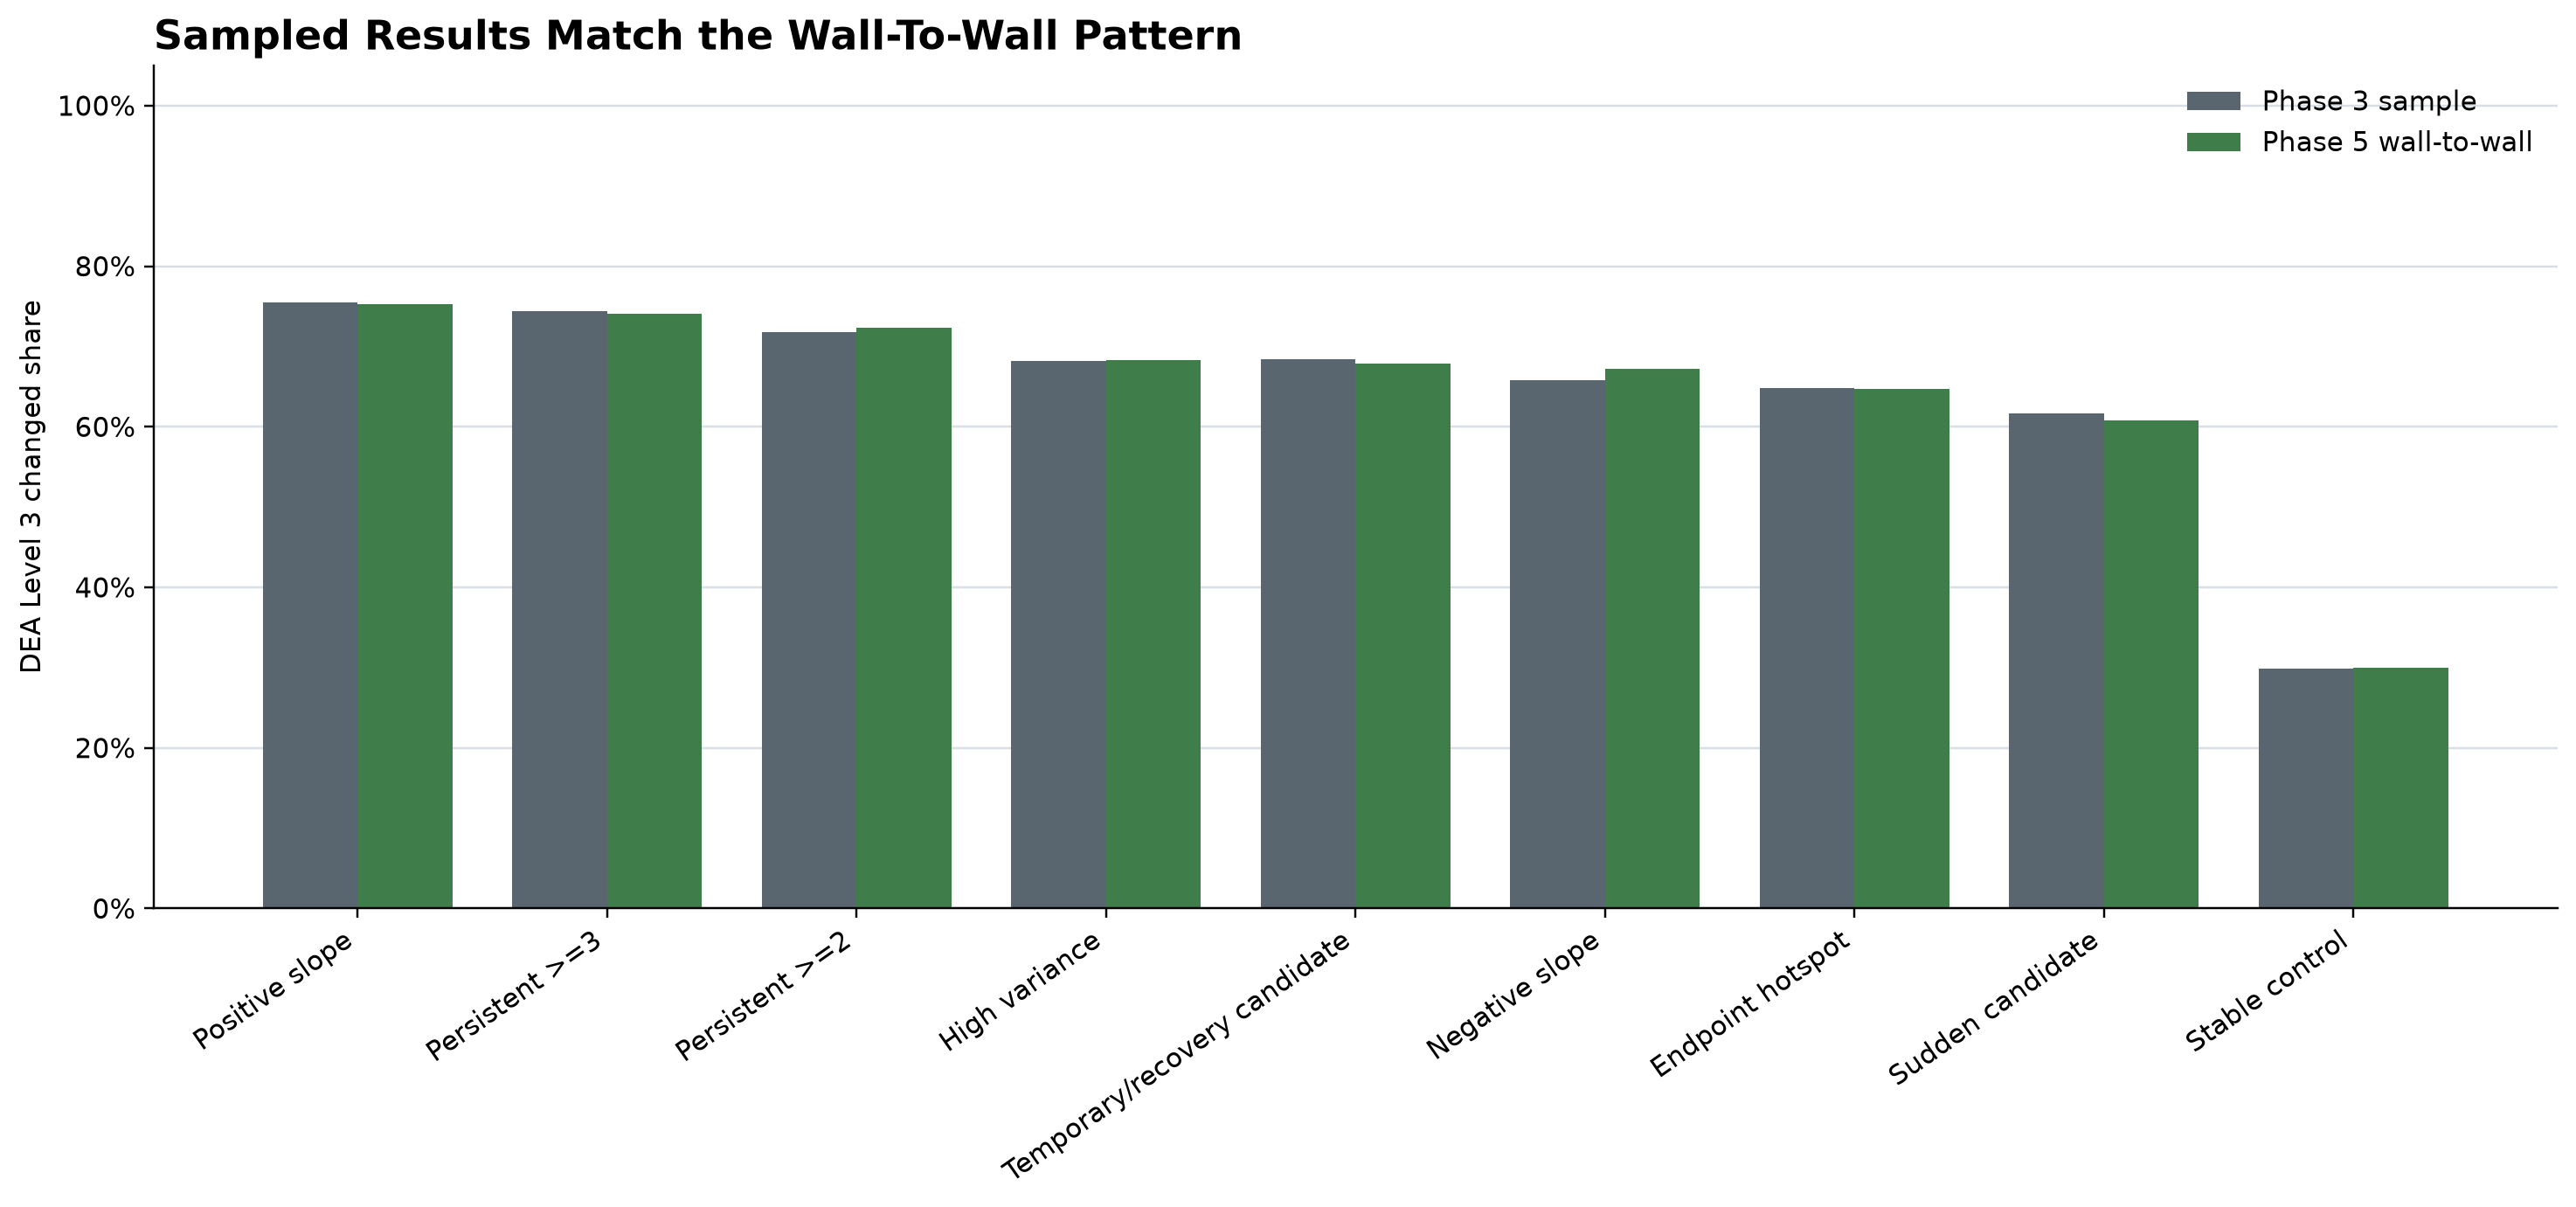
\includegraphics[width=0.95\textwidth]{fig14.png}
    \caption{Comparison between sample-based and wall-to-wall DEA Level 3 changed shares. The similarity between the two results indicates that the sampled analysis captured the main category-level pattern observed across the full raster stack.}
    \label{fig:sample_wall_to_wall_comparison}
\end{figure}

\section{DEA Transition and Sequence Characterization}

In addition to measuring whether a DEA class change occurred, the analysis summarized what broad land-cover transitions were most common within the embedding-derived categories. The simplest transition summary compared the DEA Level 3 class in 2017 with the DEA Level 3 class in 2024. This endpoint transition analysis provided a compact description of broad start-to-end land-cover change. Across the categories, the largest transition counts were associated with stable cultivated vegetation, stable natural vegetation, natural terrestrial vegetation to cultivated terrestrial vegetation, and cultivated terrestrial vegetation to natural terrestrial vegetation.

Figure~\ref{fig:top_dea_transitions} shows the dominant DEA Level 3 endpoint transitions. The prominence of natural-to-cultivated and cultivated-to-natural transitions indicates that many embedding-derived change signals are associated with changes between broad vegetation land-cover groups. Transitions to artificial surface were also detected, although they represented a smaller component of the overall transition structure. This result is consistent with the interpretation that the embedding-derived hotspots are not a single type of landscape change, but instead include multiple broad land-cover histories.

As with the category summaries, these transition counts are intended to describe the dominant transition patterns across behavioural categories. Because the categories can overlap, the counts should be interpreted as comparative summaries of category-associated transitions rather than as mutually exclusive counts of unique pixels.

\begin{figure}[H]
    \centering
    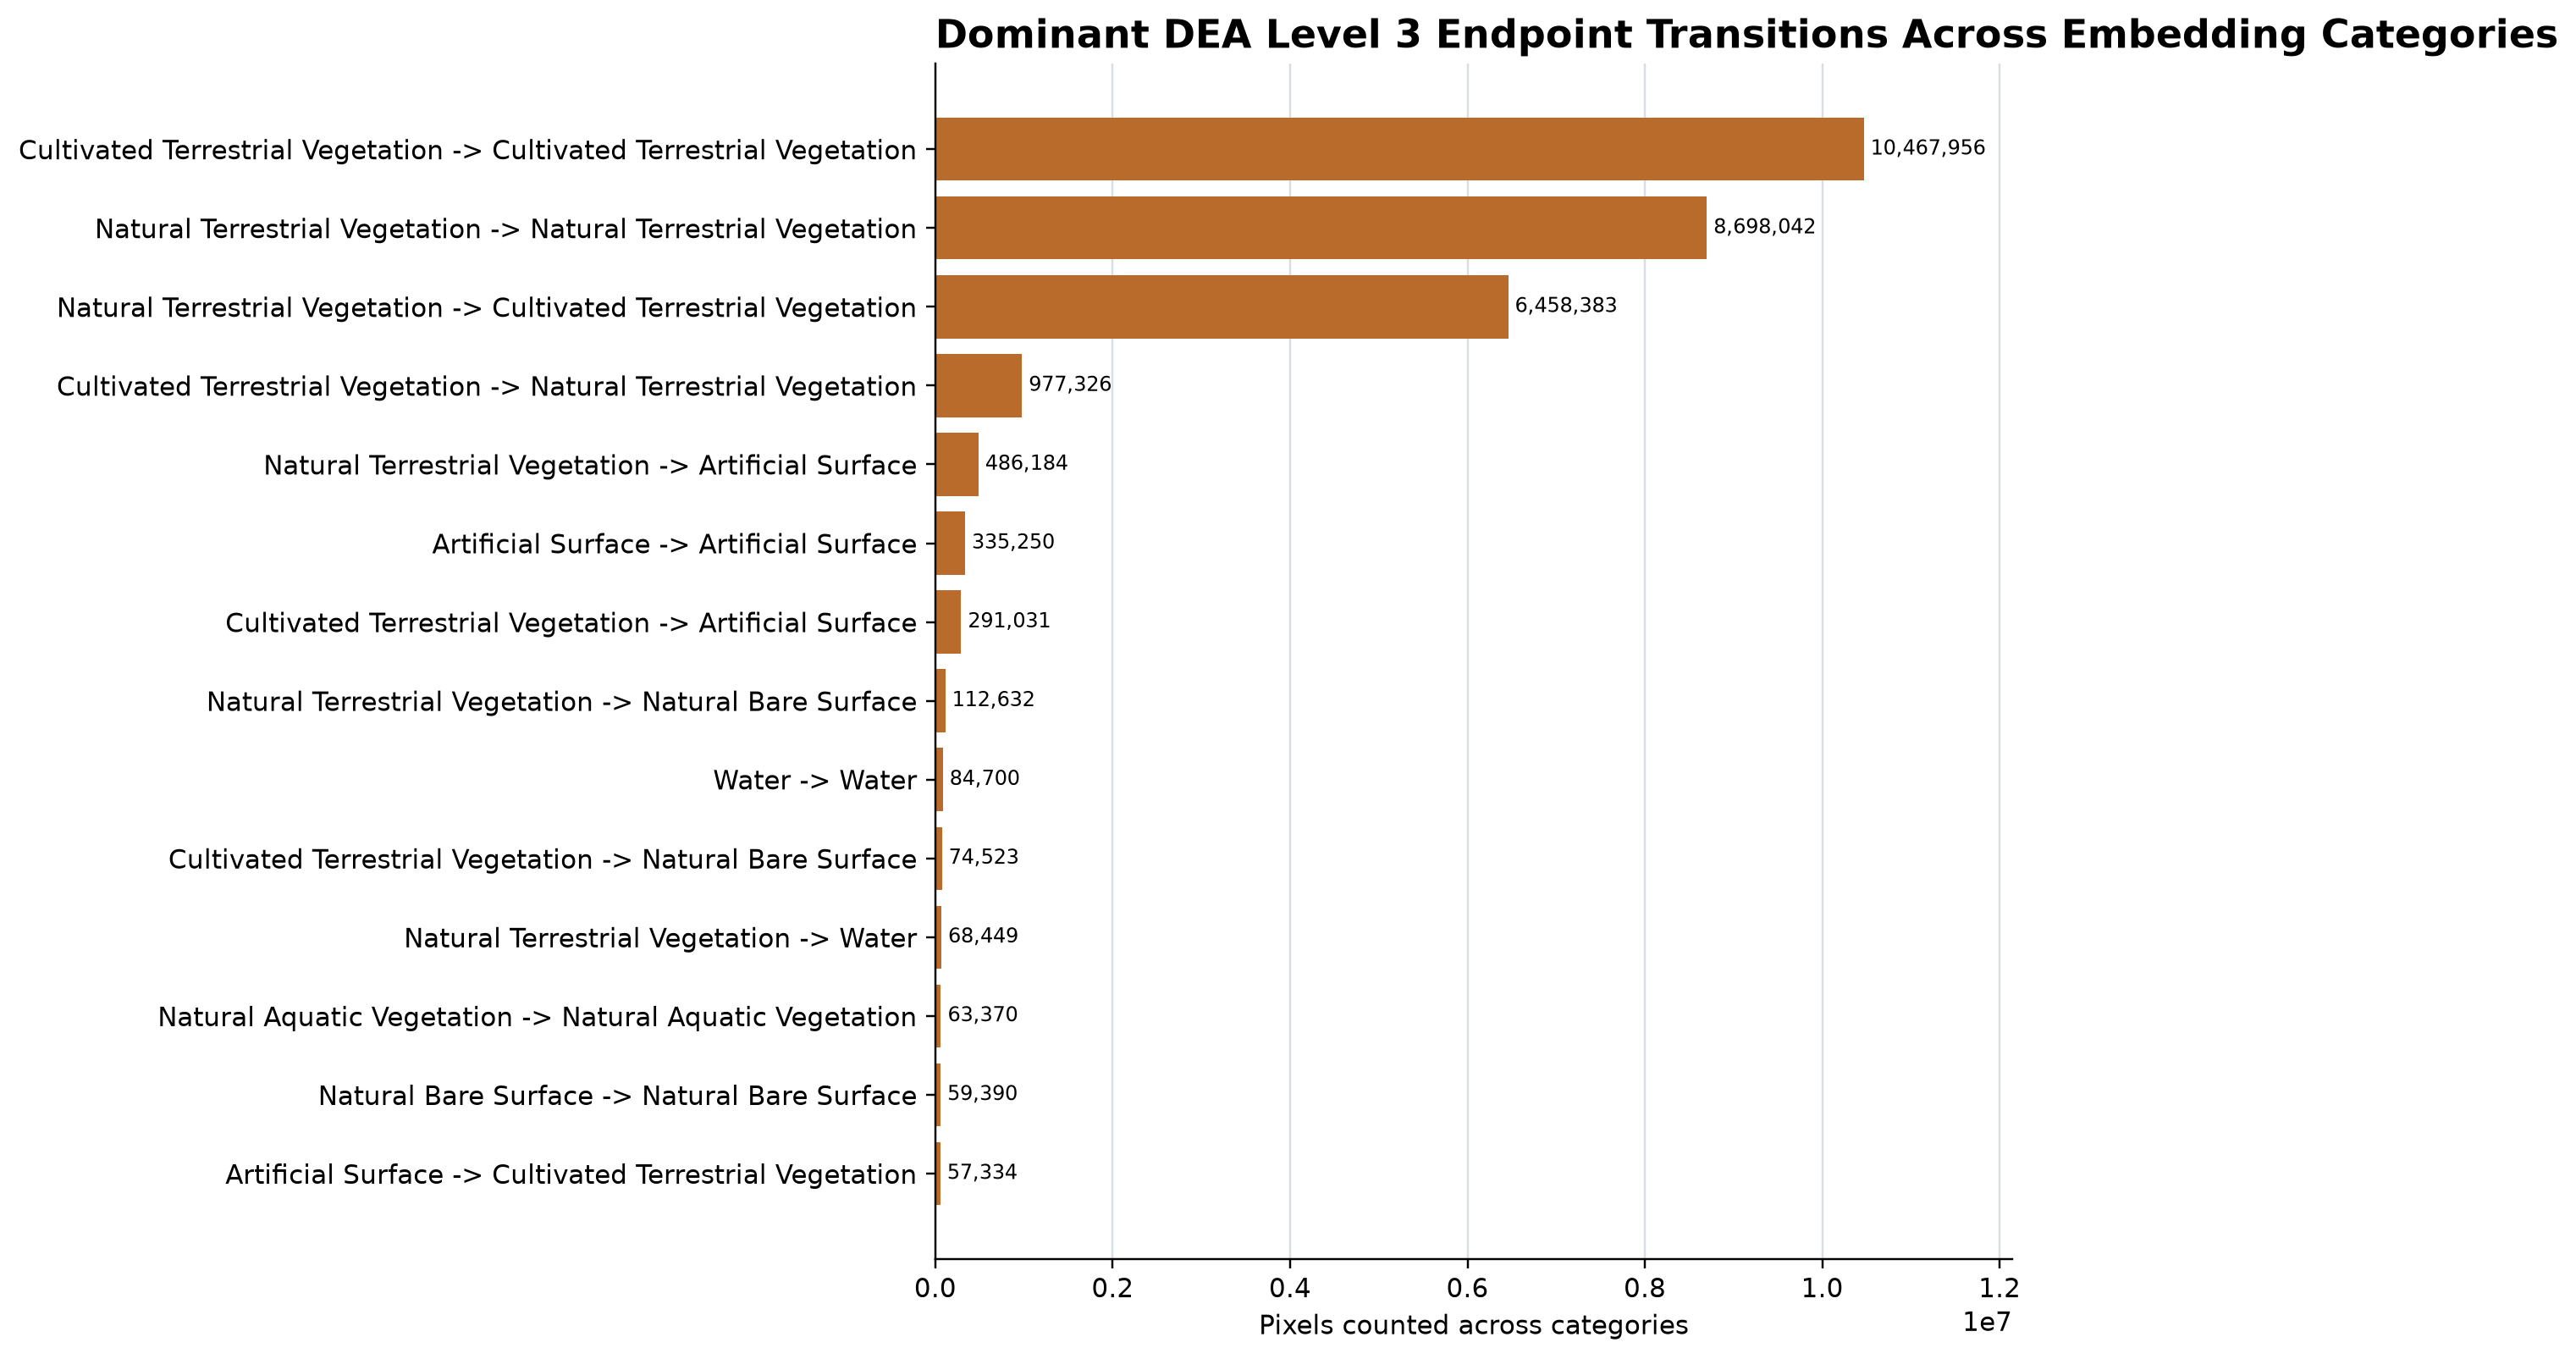
\includegraphics[width=0.95\textwidth]{fig15.png}
    \caption{Dominant DEA Level 3 endpoint transitions associated with the embedding-derived behavioural categories. Vegetation-related transitions dominate the summary, while artificial-surface transitions are present but smaller in magnitude.}
    \label{fig:top_dea_transitions}
\end{figure}

Endpoint transitions provide a useful summary, but they do not capture the full temporal behaviour of each pixel. For example, a pixel could start and end as the same DEA Level 3 class while still changing during the intervening years. To capture this behaviour, the annual DEA labels from 2017 to 2024 were also summarized as sequence types. These sequence types distinguish stable locations, transitions between natural and cultivated vegetation, transitions to or from artificial surface, water or bare-surface involvement, and cases where a pixel changed temporarily before returning to its starting class.

Figure~\ref{fig:dea_sequence_types} shows the dominant DEA Level 3 sequence types. The largest sequence type was temporary or return-to-start behaviour, indicating that many pixels experienced at least one DEA class change during the study period but returned to their initial Level 3 class by 2024. Natural-to-cultivated vegetation transitions were also common, followed by stable natural and stable cultivated sequences. This sequence-based summary is important because it shows that the embedding-derived behavioural categories are associated not only with endpoint land-cover transitions, but also with more complex annual land-cover histories.

\begin{figure}[H]
    \centering
    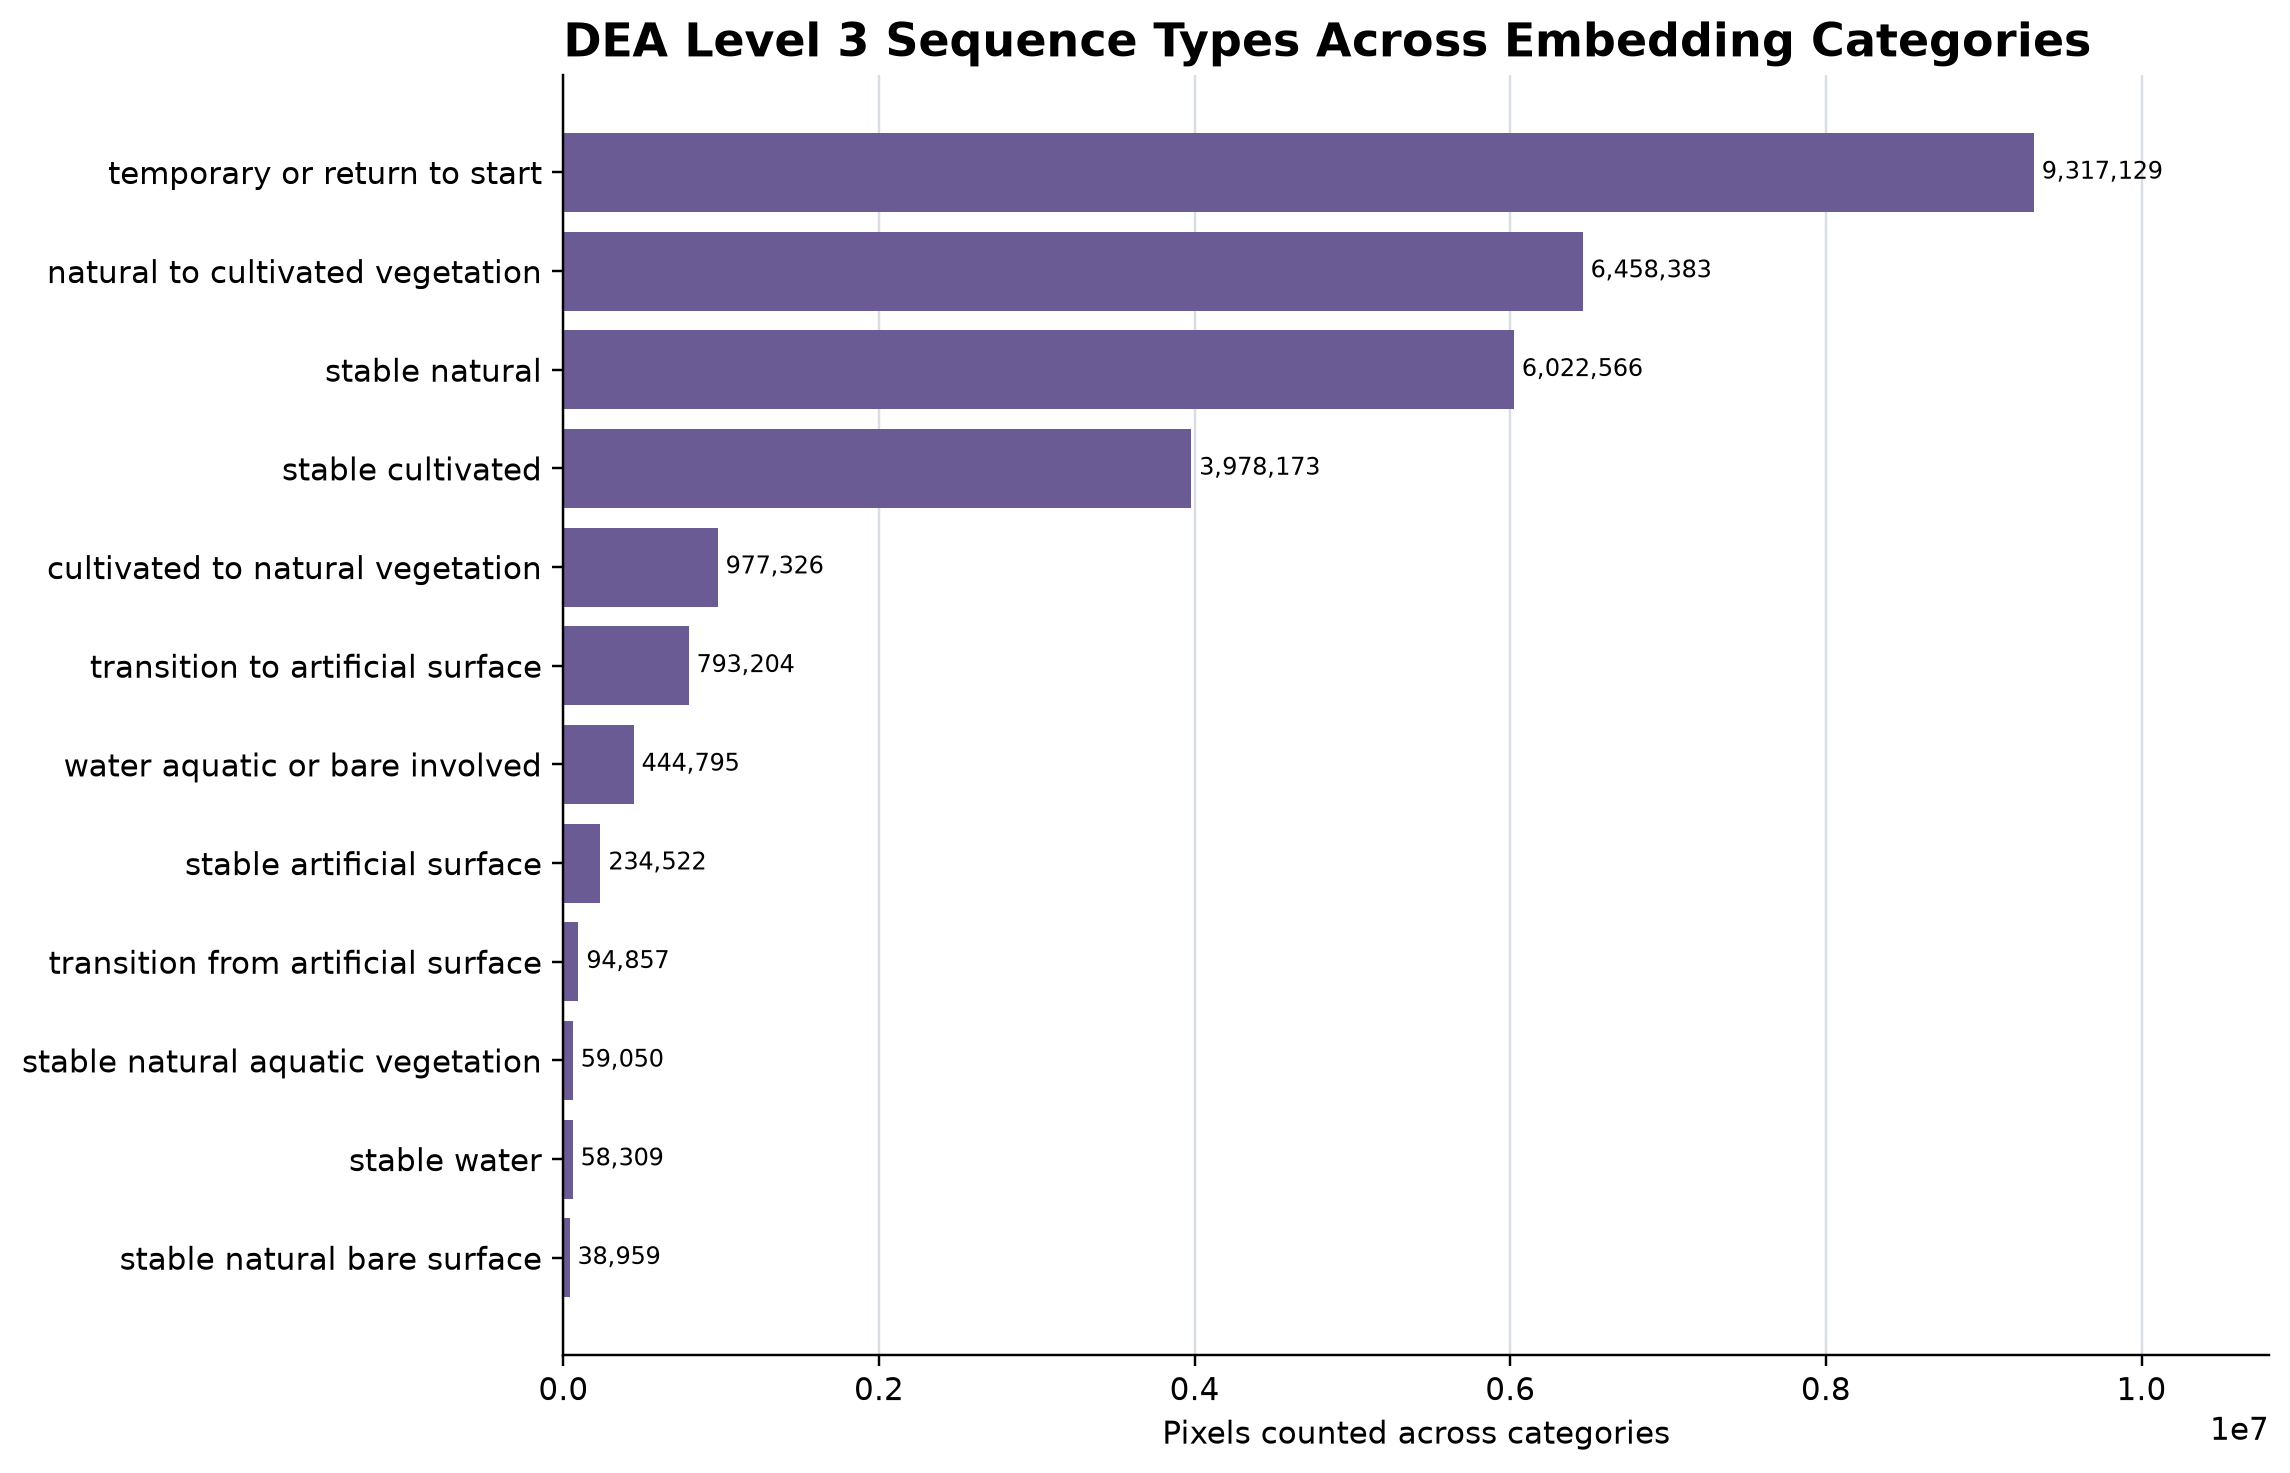
\includegraphics[width=0.85\textwidth]{fig16.png}
    \caption{DEA Level 3 sequence types across embedding-derived behavioural categories. Sequence summaries capture annual behaviour across the full 2017--2024 period rather than only the start and end classes.}
    \label{fig:dea_sequence_types}
\end{figure}

\section{Temporal and Spatial Interpretation}

The temporal metrics derived from the embedding products were designed to describe not only the magnitude of change, but also when strong change occurred. To evaluate whether these timing metrics were broadly consistent with DEA Land Cover histories, the first year of DEA Level 3 change was compared with the embedding-derived maximum change year and first hotspot year. A match was counted when the DEA first-change year occurred within one year of the corresponding embedding timing metric. This comparison was not intended to be a strict accuracy test, because DEA Land Cover and Satellite Embedding V1 measure different properties of the landscape at different thematic resolutions. Instead, it was used as a consistency check between independent temporal signals.

Figure~\ref{fig:timing_alignment} summarizes the timing alignment results. Persistent categories showed relatively strong alignment between DEA first-change year and first hotspot year, particularly for pixels with persistence greater than or equal to three years. Negative-slope pixels showed stronger alignment with maximum change year. These patterns suggest that different embedding-derived behavioural categories relate to DEA timing in different ways, which is consistent with the broader idea that the temporal metrics capture distinct modes of landscape behaviour.

\begin{figure}[H]
    \centering
    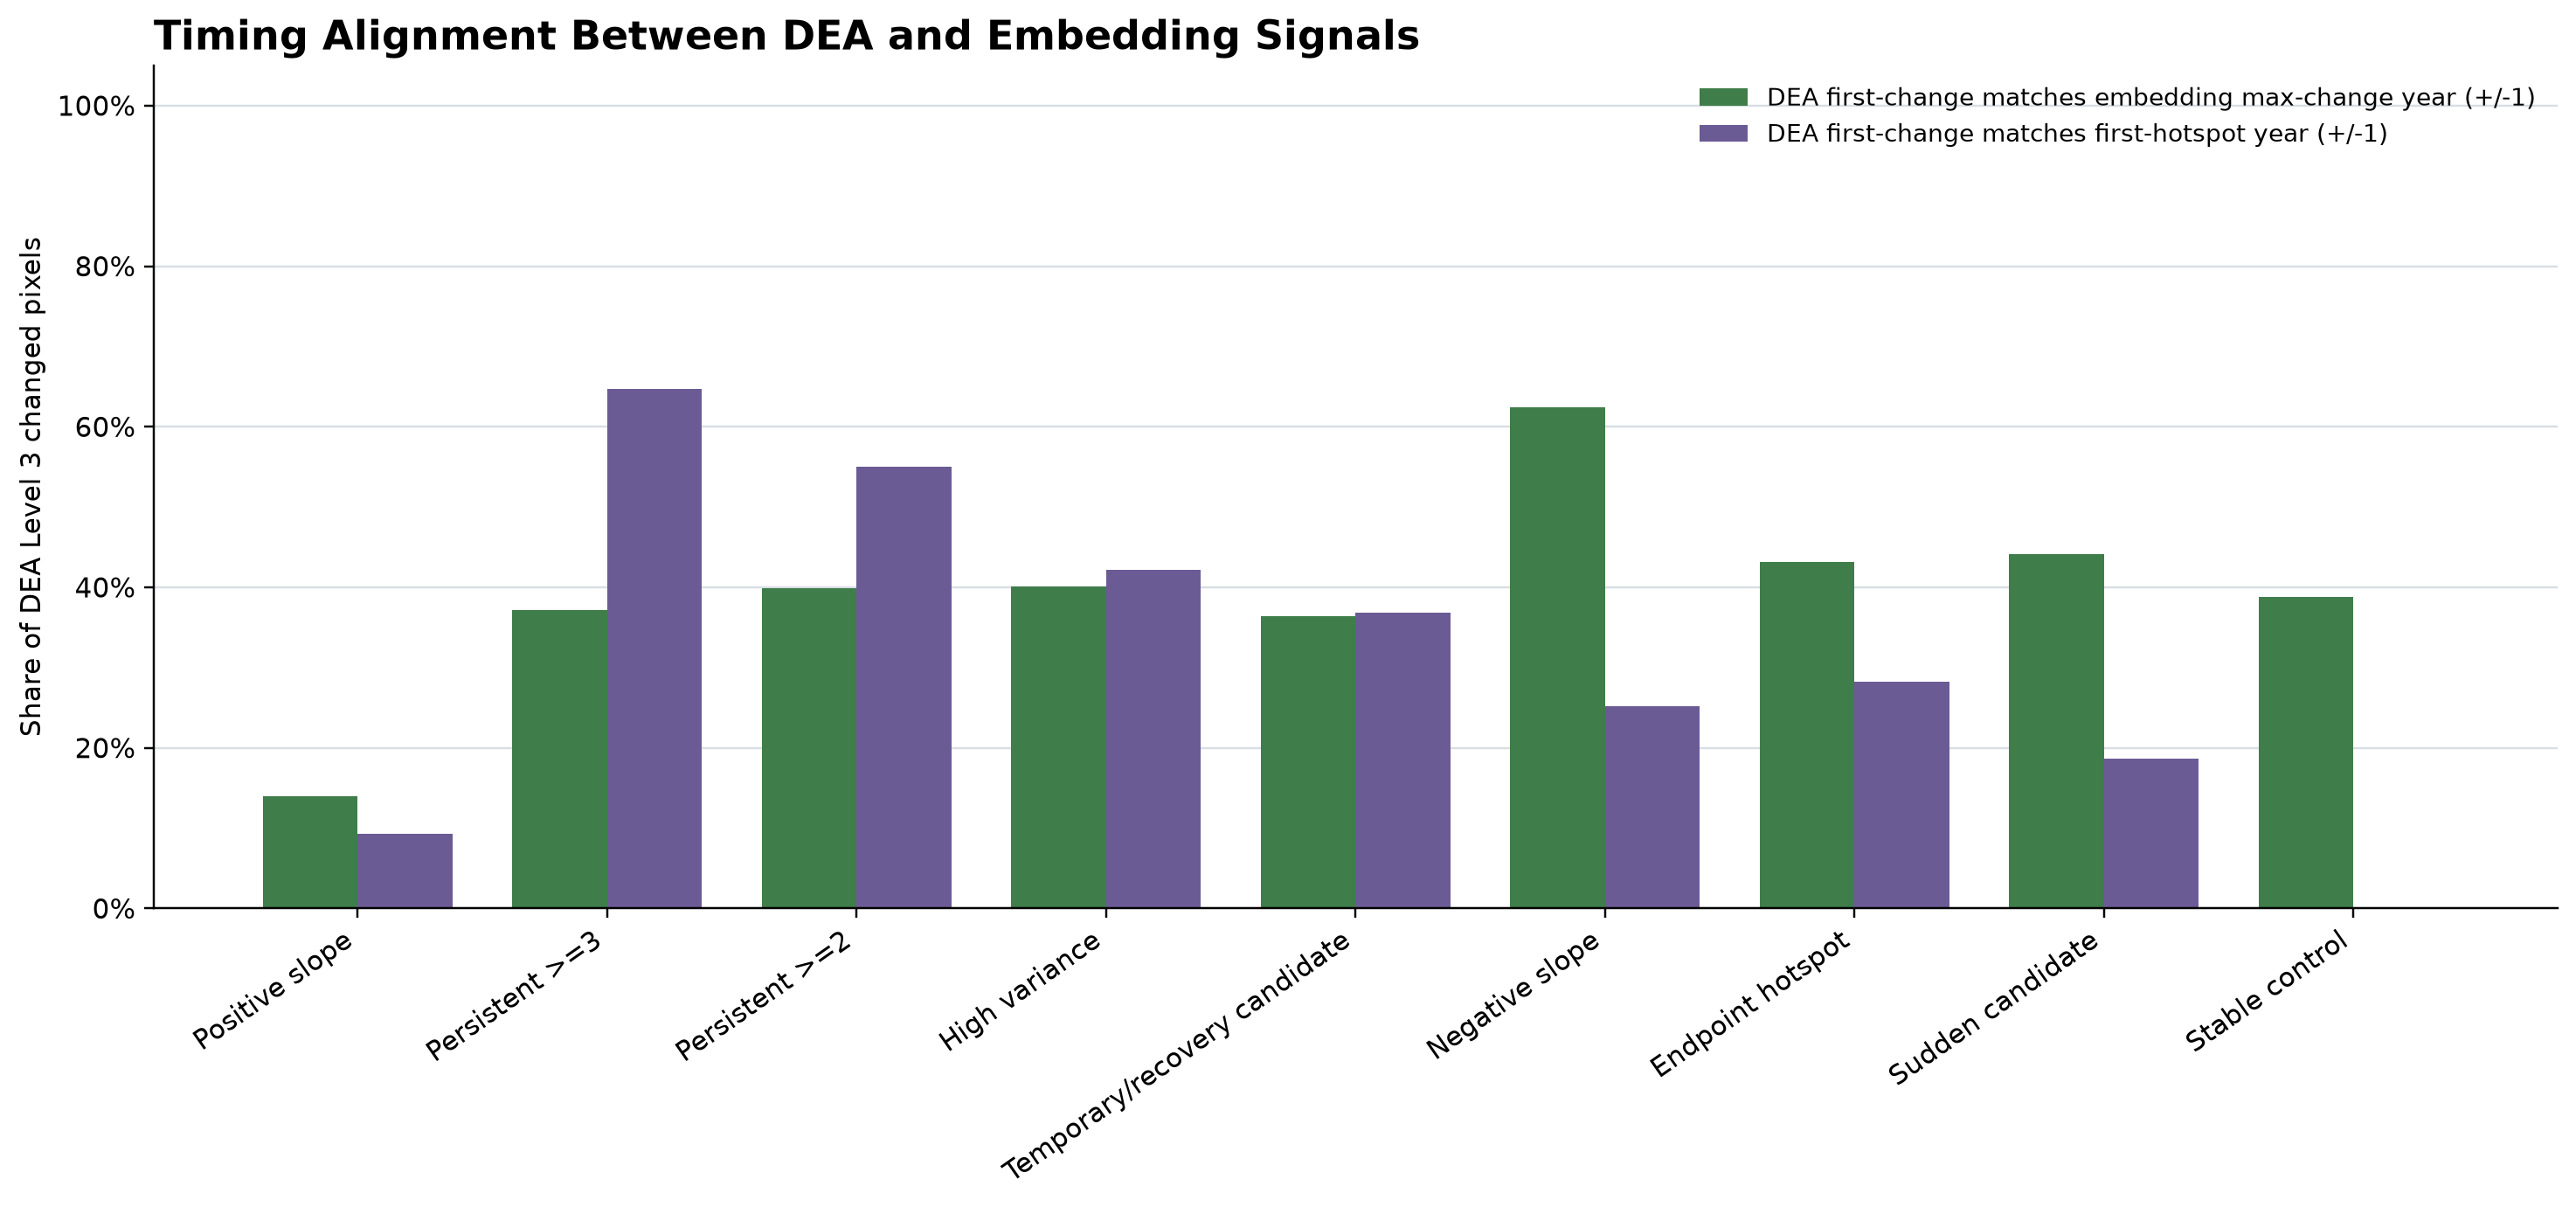
\includegraphics[width=0.95\textwidth]{fig17.png}
    \caption{Temporal alignment between DEA first-change year and embedding-derived timing metrics. The values represent the share of DEA Level 3 changed pixels where the DEA first-change year occurred within one year of the embedding timing metric.}
    \label{fig:timing_alignment}
\end{figure}

The final stage of the current analysis focused on spatial visualization. While the preceding summaries quantify relationships between embedding categories and DEA land-cover histories, spatial maps are needed to understand where these relationships occur across the Bass Coast landscape. Figure~\ref{fig:dea_sequence_map} shows DEA Level 3 sequence types across the full study area. This map provides a spatial view of broad land-cover histories, including stable natural areas, stable cultivated areas, natural-to-cultivated transitions, cultivated-to-natural transitions, temporary or return-to-start behaviour and areas involving water, bare surface or aquatic vegetation.

\begin{figure}[H]
    \centering
    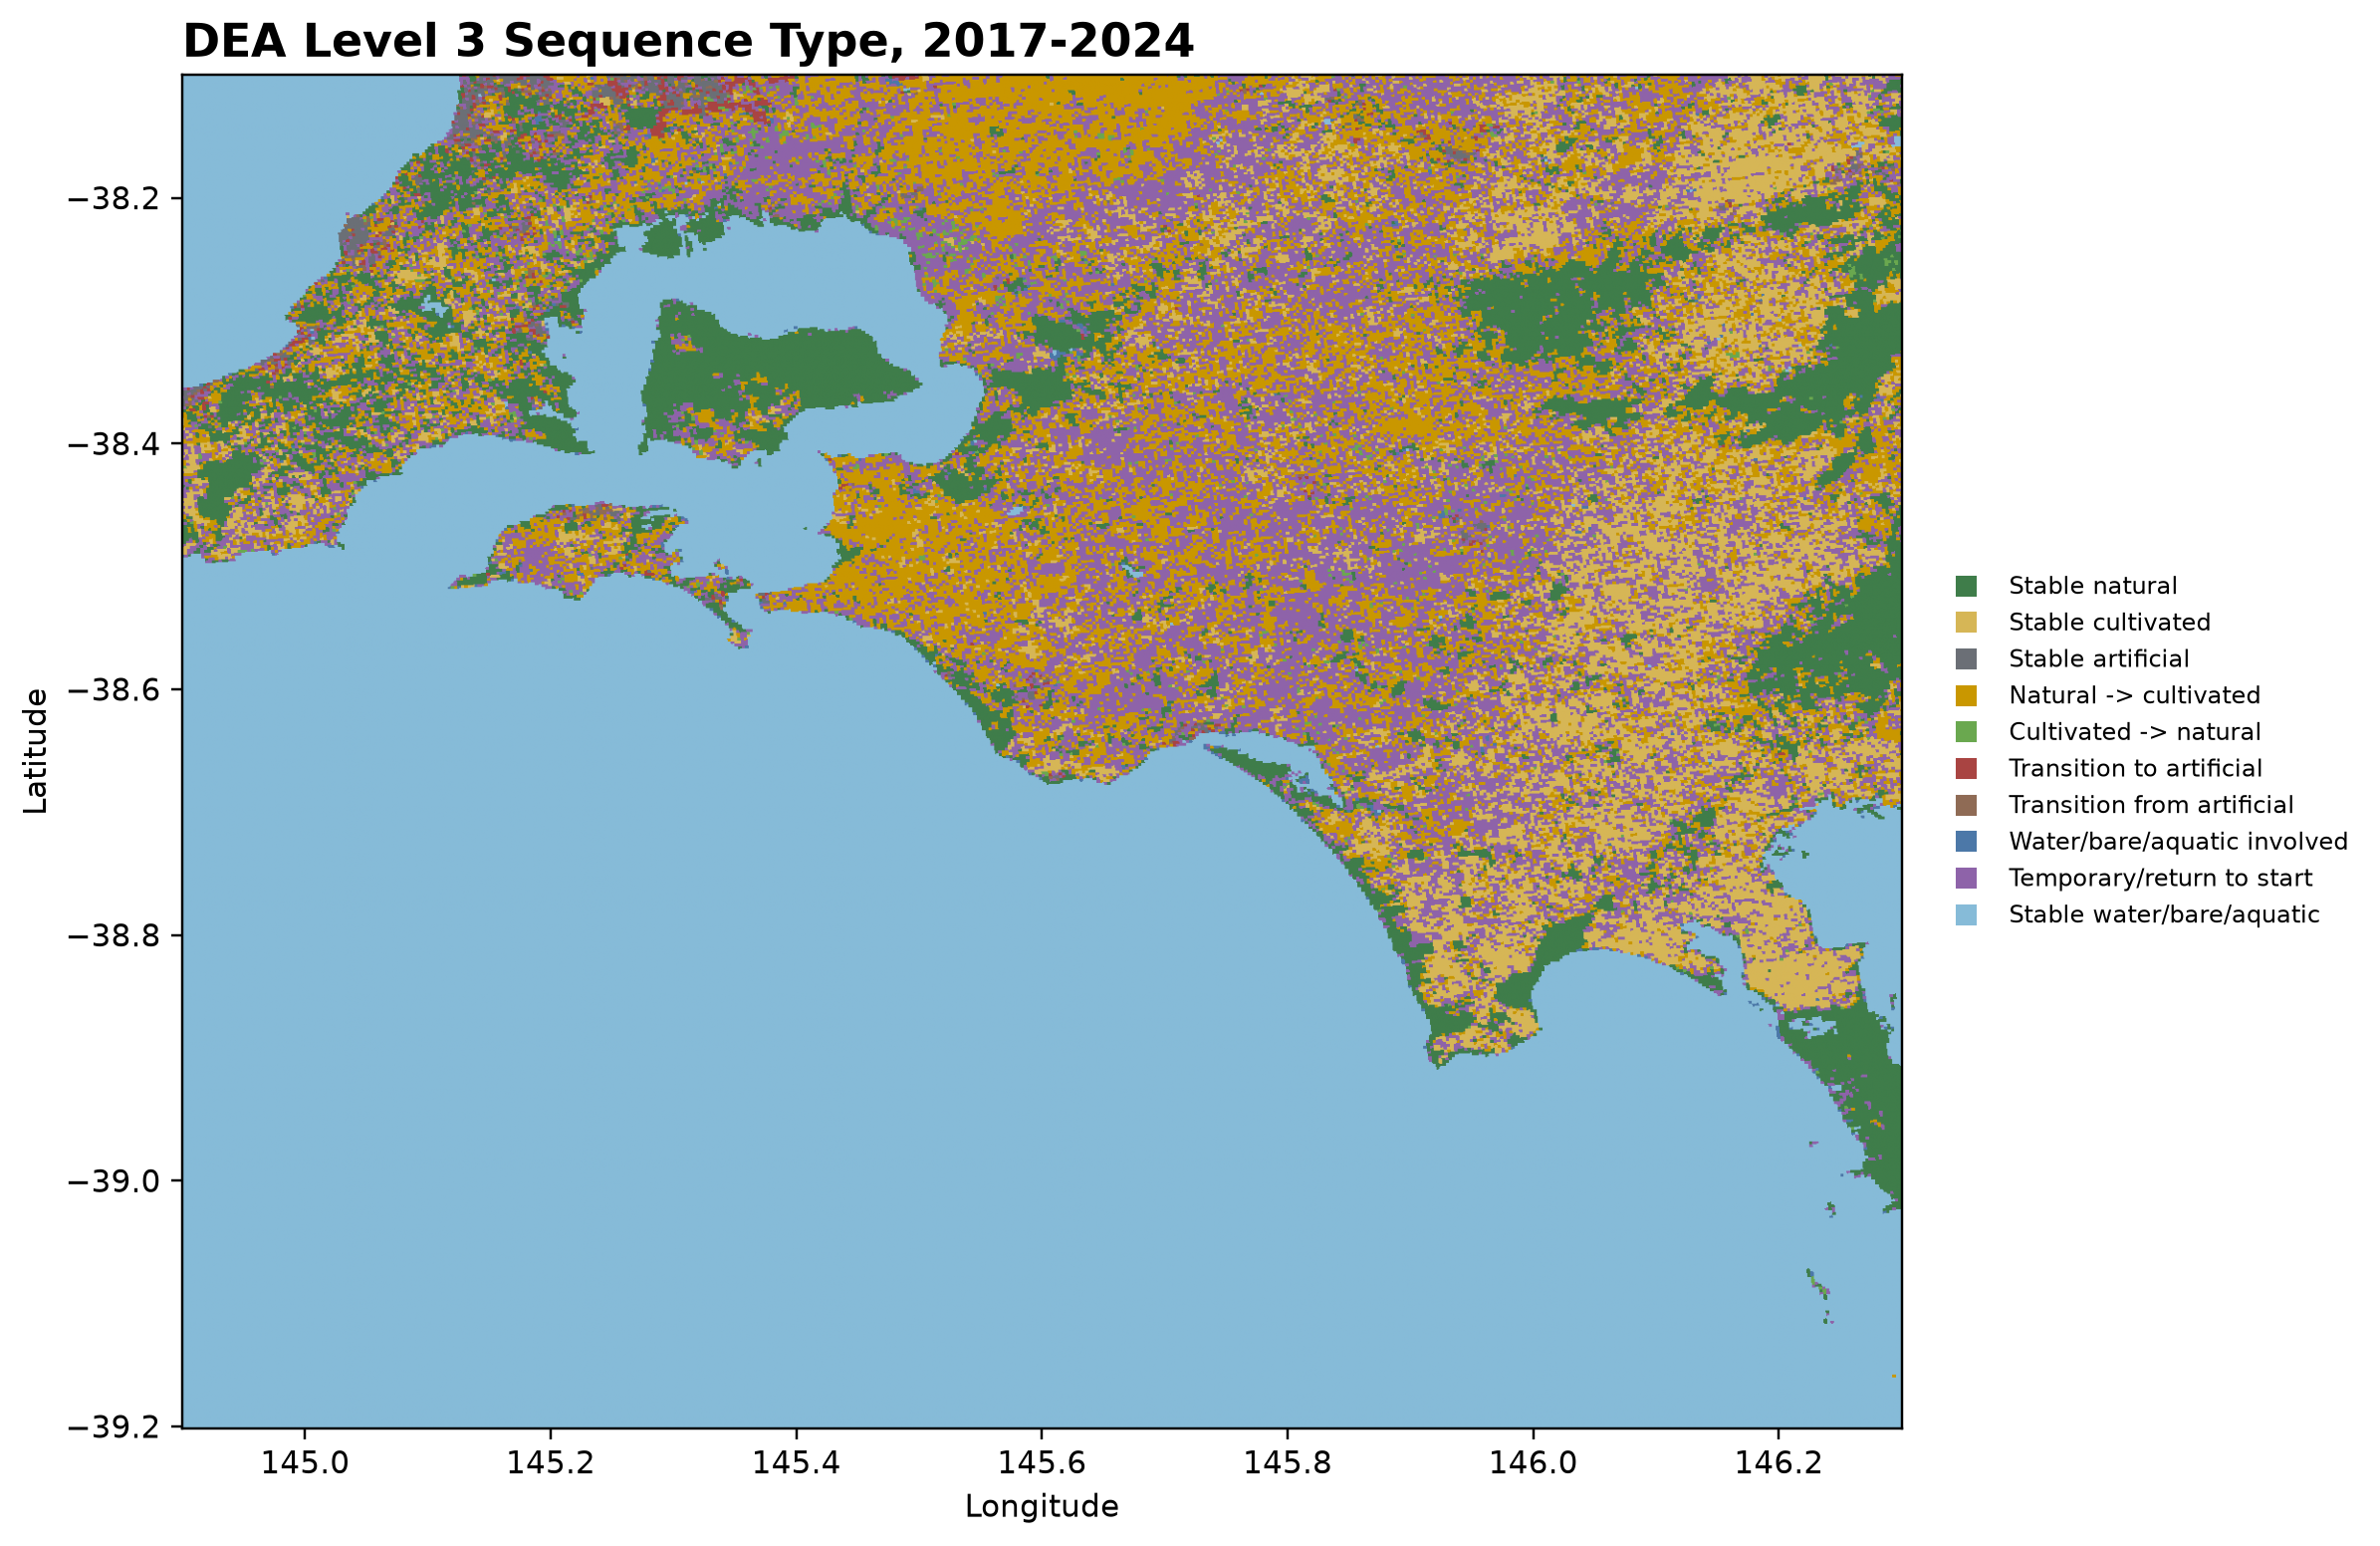
\includegraphics[width=0.85\textwidth]{fig18.png}
    \caption{Spatial distribution of DEA Level 3 sequence types across the Bass Coast study area. The map summarizes broad annual land-cover histories from 2017 to 2024.}
    \label{fig:dea_sequence_map}
\end{figure}

Figure~\ref{fig:hotspot_dea_overlay} links the embedding-derived endpoint hotspot layer with the DEA sequence classification. In this visualization, only endpoint hotspot pixels are shown, and each hotspot is coloured by its associated DEA Level 3 sequence type. This provides a direct visual connection between the AI-derived change map and the external land-cover history layer. The overlay demonstrates that hotspot areas are associated with a mixture of DEA histories, including vegetation transitions, temporary or return-to-start behaviour, stable land-cover classes and smaller areas involving artificial-surface transitions.

\begin{figure}[H]
    \centering
    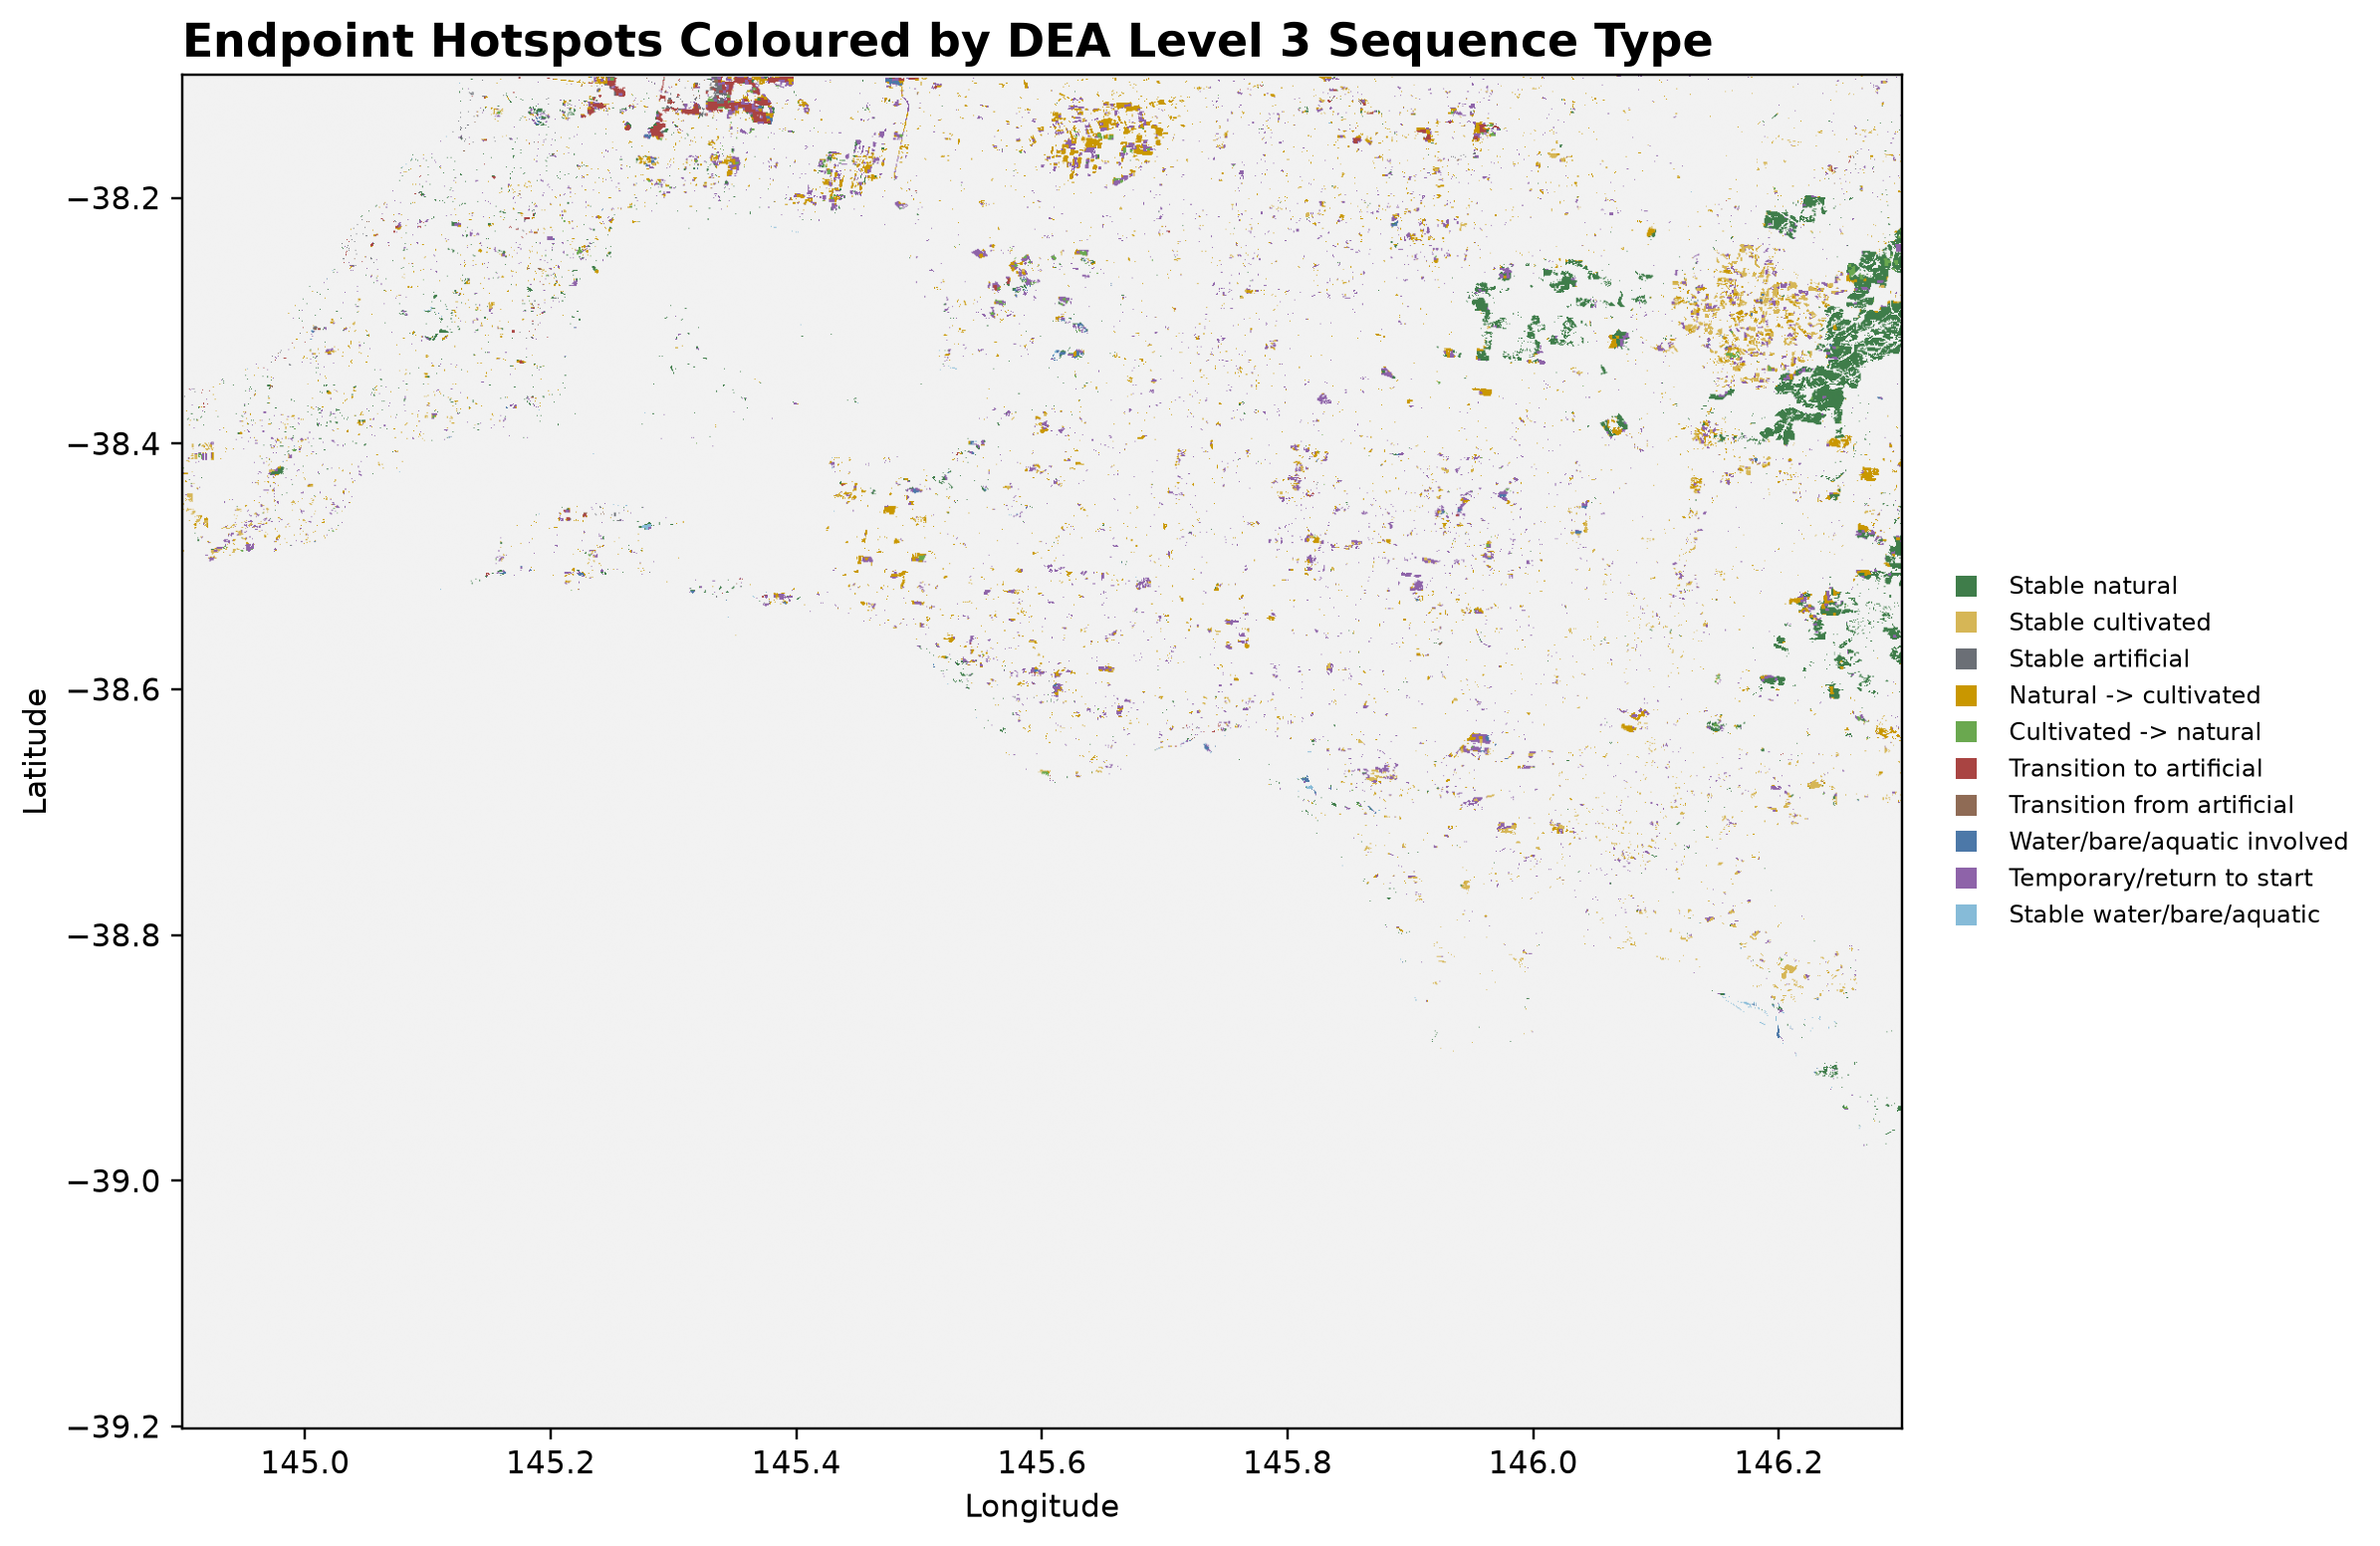
\includegraphics[width=0.85\textwidth]{fig19.png}
    \caption{Endpoint hotspot pixels coloured by DEA Level 3 sequence type. This overlay connects embedding-derived hotspot locations with broad DEA land-cover histories.}
    \label{fig:hotspot_dea_overlay}
\end{figure}

\section{Current Findings and Limitations}

The work completed to date represents an important milestone in the development of the AusHabitat change-monitoring framework for the Bass Coast case study. The workflow has progressed from embedding-based hotspot detection to temporal behaviour characterization, sample-based external enrichment, wall-to-wall DEA Land Cover summarization and spatial visualization. Together, these stages show that Satellite Embedding V1 can be used not only to identify areas of strong change, but also to characterize different temporal patterns of change and relate those patterns to independent land-cover histories.

The main finding from the DEA integration is that embedding-derived change categories are strongly enriched for DEA-observed land-cover change relative to stable controls. In the wall-to-wall analysis, most change-oriented behavioural categories had DEA Level 3 changed shares between approximately 61\% and 75\%, while the stable-control category had a changed share of approximately 30\%. This pattern was already visible in the sampled analysis and was confirmed across the full raster stack. The consistency between the sampled and wall-to-wall results suggests that the behavioural categories derived from the embedding metrics capture meaningful landscape dynamics rather than arbitrary numerical groupings.

The transition and sequence summaries also show that the embedding-derived change signals are associated with multiple broad land-cover histories. Vegetation-related transitions were dominant, particularly transitions between natural terrestrial vegetation and cultivated terrestrial vegetation. Artificial-surface transitions were present but smaller in magnitude. The sequence analysis further showed that many pixels experienced temporary or return-to-start behaviour, highlighting the value of annual time-series analysis rather than relying only on 2017-to-2024 endpoint comparisons.

Several limitations should be kept in mind when interpreting these results. First, DEA Land Cover provides broad categorical land-cover labels, not direct causal explanations. A DEA transition can indicate that a location changed from one broad land-cover class to another, but it does not by itself explain why that change occurred. Second, DEA Land Cover and Satellite Embedding V1 differ in spatial resolution and thematic structure. DEA labels were used as broad contextual information aligned to the embedding grid, but this should not be interpreted as independent 10 m land-cover classification. Third, the behavioural categories remain rule-based temporal candidates. They are useful for organizing and testing embedding-derived change patterns, but they should not yet be interpreted as definitive ecological classes such as degradation, restoration, urbanization or agricultural conversion without further supporting evidence.

Despite these limitations, the current results demonstrate that the framework can connect AI-derived change signals with independent land-cover histories in a scalable and interpretable way. This provides a stronger basis for understanding the environmental meaning of embedding-derived hotspots and establishes a clearer technical record of the progress achieved so far.

\end{document}
